\documentclass[10pt]{article}
\usepackage{commands}
\hypersetup{colorlinks = true}

\begin{document}
\begin{tcolorbox}
  \begin{center}
  \begin{Large}
    \textbf{PHYS 410 Computational Physics Notes} \\
    \vspace{5pt}
  \end{Large}
  \begin{large}
        Tobias Faehndrich \\
\vspace{5pt}
    \emph{This document was last edited on \today}
  \end{large}
  \end{center}
\end{tcolorbox}

\begin{center}
  \textbf{Introduction:}

Notes written while following the upper-level undergraduate course taught at the University of British Columbia in the Fall 2023 semester by Dr. Matt Choptuik. If any errors are found in the notes, feel free to email me at \href{mailto:tobias.faehndrich@gmail.com}{tobias.faehndrich@gmail.com}. Overleaf formatting was copied from Rio W.

\end{center}
\addtocontents{toc}{\protect\hypertarget{toc}{}}
\tableofcontents

\newpage
\def \secname {Syllabus}

\section[\secname]{\hyperlink{toc}{\secname}}


\newpage
\def \secname {Programming Basics}

\section[\secname]{\hyperlink{toc}{\secname}}


\textbf{Relational and Logical Operators:}

\begin{itemize}
    \item Matlab follows C approach
    \item 0 for false and 1 for true (for evaluating expressions)
    \item Relational: tilda equal (not equal), and then normal ones like >, <, etc...
    \item Logical: and symbol, | or symbol, tilda is not, and then double and symbol is short circuit, and double | is short circuit OR
\end{itemize}

\textbf{Control Structures}

Selection/Conditional:
\begin{itemize}
    \item  if-elseif-else-end statements
    \item no colons 
    \item end conditional with end
\end{itemize}

Iteration (repetition, and loops)

FOR
\begin{itemize}
    \item for <var> = <first> : <step> : <last> do something and then end
    \item without step, auto is step = 1
    \item can also give vector to iterate through or linspace
    \item again need to end
\end{itemize}

WHILE
\begin{itemize}
    \item While the expression is true keep evaluating code block and then end when it is False
    \item can use break to get out of the innermost loop, if it is in the general code block, it will stop the running of the script
\end{itemize}

CONTINUE
\begin{itemize}
    \item used within a loop to short circuit the execution of the loop body and proceed to the next iteration
\end{itemize}

RETURN
\begin{itemize}
    \item causes an immediate return of a script or function to the invoking environment
\end{itemize}



\textbf{Programming Units: Scripts and Functions}
\begin{itemize}
    \item in linux command you can call a script or a function script with the .m extension
    \item arb num of inputs and outputs
    \item function name(args...) for 0 output
    \item function output = name(args...) for 1 outputs
    \item function [out1, out2 .... outn] = name(in1, in2, ... inm) for n and m outputs and inputs
    \item Ideally name of function is the same as the name of the script
    
\end{itemize}




\newpage
\def \secname {Floating Point Arithmetic and Stability}

\section[\secname]{\hyperlink{toc}{\secname}}

\textbf{1. Floating Point Arithmetic}

1.1 Some Definitions
\begin{itemize}
    \item To start
    \[ a = \text{some exact (reference) value}\]

    \[\hat{a} = \text{some approx of a (floating point of a)}  \]

    \item Absolute Error (error)
    \[ e_{ABS} = a - \hat{a} \text{ or }\hat{a}-a \text{, doesn't matter}\]
    \item Relative Error 
    \[e_{REL} = \frac{a-\hat{a}}{|a|} \text{ For } a \neq 0 \]

    \item Note this difference is important for HW1
\end{itemize}



1.2 IEEE 64-bit floating point arithmetic
\begin{itemize}
    \item 53 bits mantissa, II bits exponents, base-2 representation sign-bits for both mantissa / exponents.

    \item numbers in the range around $2\times 10^{-300}$ to $1\times 10^{+300}$ with approx 16 decimal digits precision.

    \item $\frac{1}{f_{min}} < f_{MAX} $ So we don't have overflow with respect to reciprocal
    \item Special (exceptional) values:
    \begin{itemize}
        \item infinity (ex 1.0/0.0)
        \item nan (not a number) (ex. 0.0/0.0)
        \begin{itemize}
            \item nan is contagious -- nan (* / + -) makes anything equal nan
        \end{itemize}
    \end{itemize}
\end{itemize}

1.3 Machine Precision / Machine $\epsilon$

\begin{itemize}
    \item Smallest $\epsilon > 0$ such that
    \[1+\epsilon \neq 1 \qquad \epsilon \approx 10^{-8}\]
    In the floating point model.
\end{itemize}


1.4 Round Off error: Catastrophic loss of precision

\begin{itemize}
    \item Multiplies/divides: relatively benign, relative error grow like $\sqrt{n}$ where n is the number of operations
    \item addition/subtraction: serious problem when subtracting x/y with $x\approx y$
    \item for example 3.6326-3.6325=0.0001
    \item \[\frac{f(x+h)-f(x)}{h}\] as h approaches 0
    \item plot ln(abs error) vs |ln(h)| and we see when h is not 0 there is a catastrophic loss of precision.
\end{itemize}

1.5 Stability / Numerical Stability
\begin{itemize}
    \item Consider some process / algorithm
    \[u(x) \rightarrow y\]
    where x is the continuum variables
    \item Floating point representation
    \[\hat{u}(\hat{x}) \rightarrow \hat{y}\]
    m,n component vectors

    \item Heuristic (non-rigorous) definition of stability:

    \item \textbf{Continuum}: If $|{x-x'}|$ is small, then so is $||u(x)-u(x')||$

    \item \textbf{Floating Point}: If $||\hat{x}\hat{x}'||$ is small, then so is $||\hat{u}(\hat{x}')-\hat{u}(\hat{x}||$

    \item Unfortunate fact: stable condition process does not imply stable floating point one.

    \item $\hat{u}$ not stable $\rightarrow$ Floating point finite precision will cause eros to rapidly accumulate, numerical process useless

    \item numerical unstable -- ill-conditioned
\end{itemize}


\newpage
\def \secname {Polynomial Interpolation}

\section[\secname]{\hyperlink{toc}{\secname}}

\subsection{Lagrange Interpolation}

\begin{itemize}
    \item Notation: $(x_j, y_j) \equiv (x_j, f(x_j)) \equiv (x_j, f_j)$
    \item Goal: Given n Data points $(x_j, f_j) \qquad j=1,2,...,n$ find (construct) unique polynomial of (maximum) degree $n-1$ passing through all data points. (Degree is the largest power of independent variable).

    \[p(x) = \sum_{i=0}^{n-1} c_i x^i \qquad \text{where c is coefficients}\]

    This is a polynomial of (maximum) degree $n-1$
    \item Once $p(x)$ is determined can use to get approximate (interpolated) values of $(f(x))$ for $x_1 \le x \le x_n$

    \item Many representations of interpolating polynomial. Lagrange approach is to take:

    \[p(x) = \sum_{j=1}^{n} f_j l_j(x) \qquad \text{where the l term is of degree n-1}\]

    Where $l_j(x)$ are characteristic polynomial satisfying

    \[l_j(x_i) = \delta_{ji}\]

    Recall the $\delta_{ji} \equiv $ Kroenicker delta where it equals 1 if $i=j$ else it equals 0

    \item Then
 \[p(x_i) = \sum_{j=1}^{n} \frac{f_jl_i(x)}{\delta_{ji}} = \sum_{j=1}^n f_j \delta_{ji} = f_i\]

    \item Building characteristic polynomial
    \[ l_j(x) = \frac{(x-x_1)(x-x_2)...(x-x_{j-1})(x-x_{j+1})...(x-x_n)}{(x_j-x_1)(x_j-2)...(x_j-x_{j-1})(x_j-x_{j+1})...(x_j-x_n)}\] 
    \item Consider $l_j(x_i)=\delta_{ji}$

    \[i=j \rightarrow \text{numerator}=\text{denominator} \qquad l_j(x_j) = 1\]

    \[i \neq j \rightarrow \text{exactly one term in numerator vanishes, so } l_i(x_i) = 0 \]


    \begin{thmbox}{Final Formula: Lagrange Interpolating Polynomial}
        \begin{equation}
            p(x) = \sum_{j=1}^n f_j l_j(x)
        \end{equation}

        \begin{equation}
            l_j(x) = \prod_{i=1, \space i \neq j}^n \frac{(x-x_i)}{(x_j-x_i)} \qquad \text{$n^2$ number of calculations}
        \end{equation}
    \end{thmbox}
    
\end{itemize}
\subsection{Barycentric Interpolation}

Related to problem of determining centre of mass for a group of particles with given positions and weights.

\begin{itemize}
    \item First, define $l(x)$
    \[ l(x) = (x-x_1)(x-x_2)...(x-x_j)...(x-x_n)\]
    Then note that numerator at $l_j$ in (2) is $l(x)/(x-x_j)$
    \item Next, define Barycentric weights by
    \[w_j = \frac{1}{\prod_{i=1, \space i \neq j}^n (x_j-z_i)}\]

    \item Then Characteristic Polynomial $l_j(x)$ is $l_j(x) = l(x) \frac{w_j}{x-x_j}$

    \item Get the first formula for:
    
    \begin{thmbox}{Barycentric Interpolation}
        \begin{equation}
            p(x) = f(x) \qquad \sum_{j=1}^n \frac{w_j}{x-x_j} f_j \qquad \text{n number of operations}
        \end{equation}
    \end{thmbox}



    \item Advantage 
    \begin{itemize}
        \item Original $O(n^2)$ calculations to eliminate at any point.
        \item Barycentric: $O(n^2)$ to compute weights, $O(n)$ to evaluate
    \end{itemize}
    
    \item Another version: let all $f_j = 1$ then from (1) AND (3)
    \[1 = \sum_{j=1}^n l_j (x) = l(x)\sum_{j=1}^n \frac{w_j}{x-x_j}\]

    \item Divide (3) by last result, cancel $l(x)$ Term

    \begin{thmbox}{Barycentric Interpolation Version 2}
        \begin{equation}
            p(x) = \sum_{j=1}^n \frac{w_j}{x-x_j} f_j / \sum_{j=1}^n \frac{w_j}{x-x_j}
        \end{equation}
    \end{thmbox}
\end{itemize}

\subsection{Numerical Example (EXAM HINT)}

!!!!!!!!!!!!!!!!!!!!!!!!!!!!!!!!!!!!!!!!!
\begin{itemize}
    \item Use (1), (2) to construct degree-2 Polynomial passing through (-1,6), (1,8), (3,34) for 
\end{itemize}

\[p(x) = \sum_{j=1}^n f_j l_j(x) \]

\[l_j(x) = \prod_{i=1, \space i \neq j}^n \frac{(x-x_i)}{(x_j-x_i)} \qquad \text{$n^2$ number of calculations}\]

\[ p(x) = 6 \frac{(x-1)(x-3)}{(-1-1)(-1-3)} + 8 \frac{(x+1)(x-3)}{(1+1)(1-3)} + 34 \frac{(x+1)(x-1)}{(3+1)(3-1)}\]

\[ p(x) = 6 \frac{(x-1)(x-3)}{8} + 8 \frac{(x+1)(x-3)}{-4} + 34 \frac{(x+1)(x-1)}{8}\]

\[ p(x) = 3\frac{(x-1)(x-3)}{4} + -2 (x+1)(x-3) + 17 \frac{(x+1)(x-1)}{4}\]


Let me check my answer by plotting the points and the result polynomial equation:


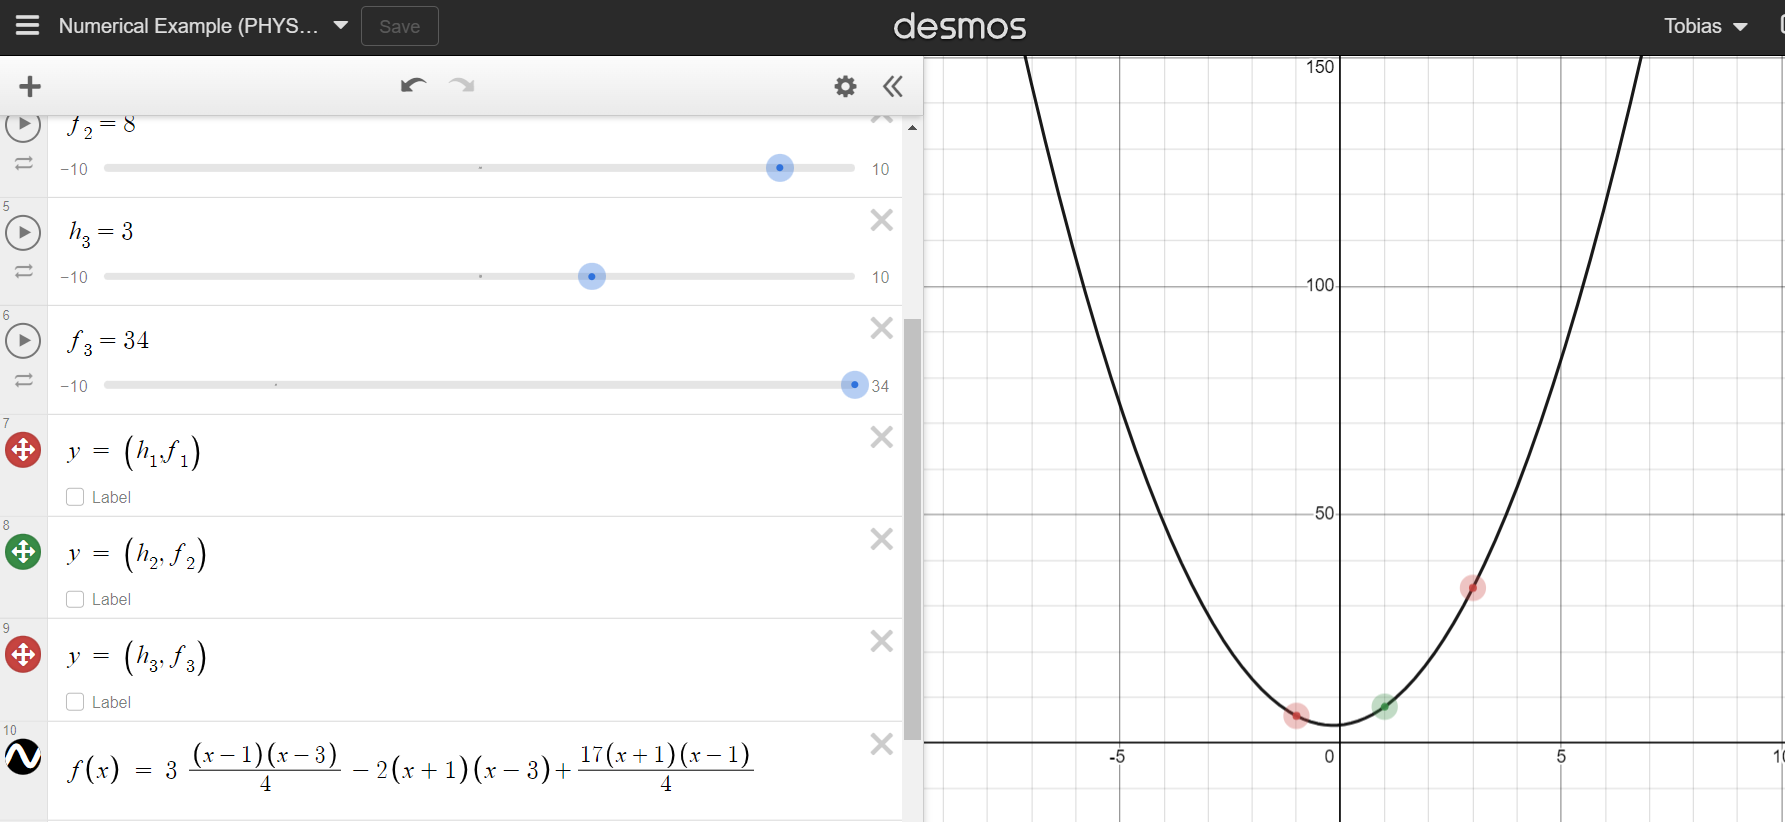
\includegraphics[width = \linewidth]{Images/NumericalExample_LagrangePolyInterp.png}

!!!!!!!!!!!!!!!!!!!!!!!!!!!!!!!!!!!!!!!!!

\subsection{Symbolic Example}
\begin{itemize}
    \item Consider 3 equi-spaced data points:
    \[(-h,f_{-1}), (0,f_0), (+h,f_1)\]

    \item Using (1), (2), Construct a lagrange interpolating polynomial and evaluate it's derivative at x=0

    \begin{equation*}
    \begin{aligned}
        p(x) &= \sum_{j=1}^3 f_j l_j(x)\\
        &= f_{-1}\frac{x(x-h)}{(-h)(-2h)} + f_0 \frac{(x+h)(x-h)}{(h)(-h)} + f_1 \frac{(x+h)(x)}{(2h)(h)}\\
        &= f_{-1} \frac{x^2-hx}{2h^2} - f_0 \frac{x^2-h^2}{h^2} + f_1 \frac{x^2+hx}{2h^2}
    \end{aligned}
    \end{equation*}

    \begin{equation*}
        \left. \frac{d(p(x)}{dx} \right\vert_{x=0} = \frac{f_1-f_{-1}}{2h} \rightarrow \text{Finite difference approximation for } f'(x)
    \end{equation*}
    
\end{itemize}



\newpage
\def \secname {Solution of non-linear equations (Root finding)}

\section[\secname]{\hyperlink{toc}{\secname}}

\begin{itemize}
    \item Consider two cases 
    \begin{enumerate}
        \item \[f(x) = 0 \qquad \text{1-D}\]
        \item \[ f(x) = 0 \qquad \text{d-D}\]
    \end{enumerate}
\end{itemize}

\subsection{ Solving nonlinear equations in one variable}

\begin{itemize}
    \item Two techniques: both presuppose info about location of root.

    \begin{enumerate}
        \item Bisection (Binary search)
        \item Newton's Method (Newton-Raphson)
    \end{enumerate}
\end{itemize}

\subsubsection{Preliminaries}

\begin{itemize}
    \item Want to find one or more roots of 

    \begin{equation}
        f(x) = 0
    \end{equation}

    \textbf{ANY} nonlinear equation can be cast in this \textbf{Canonical} form

    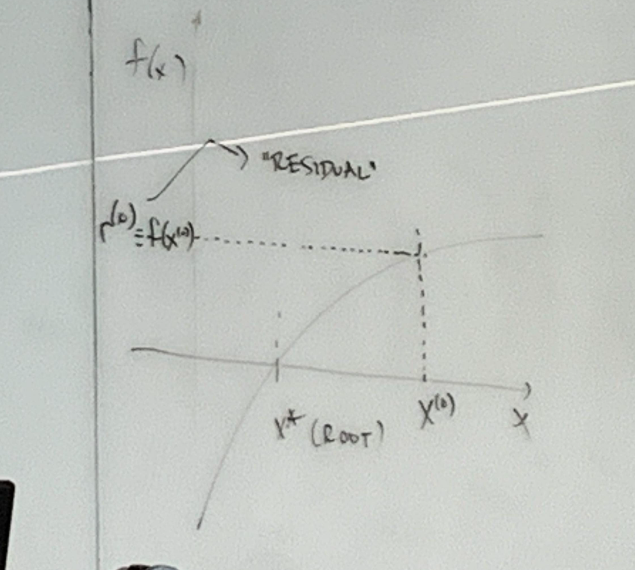
\includegraphics[width = \linewidth]{Images/410Notes_Residual.png}
    
\end{itemize}

Definition: Given Canonical equation $f(x)=0$, residual of that equation for any value x is simply $r = f(x)$

\begin{itemize}
    \item Iterative technique

    \[ x^{(0)} \rightarrow x^{(1)} \rightarrow ... \rightarrow x^{(n)} \rightarrow x^{(n+1)} \rightarrow ... \rightarrow x^{(\infty)} = x^*\]

    \[ f(x^{(0)}) \rightarrow ... \rightarrow 0 = 0\]

    \[ r^{(0)} \rightarrow ... \rightarrow 0 = 0 \]


    \item \textbf{Convergence:} Driving residual to $0\equiv$ Locating a root, $x^*$.

    \item Convergence: When do we stope iteration?

    \item Stop when
    \begin{equation}
        |\delta x^{(n)}| \equiv |x^{(n+1)} - x^{(n)}| \leq \epsilon
    \end{equation}

    for $\epsilon$ is some prescribed convergence criterion

    \item Better idea: Use relativized estimate
    
    \begin{equation}
        \frac{|\delta x^{(n)}|}{|x^{(n+1)} \leq \epsilon|}
    \end{equation}

    \item Switch over to absolute tolerance if $|x^{(n+1)}|$ becomes "too small"
    \item Motivation: Small numbers often result from "unstable" processes
\end{itemize}

\subsubsection{Bisection}

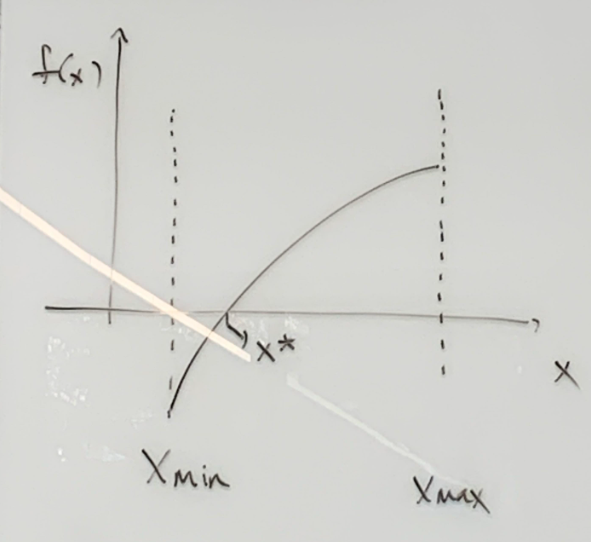
\includegraphics[width = 0.3 \linewidth]{Images/410Notes_Bisection.png}

\begin{itemize}
    \item \textbf{Demand} that $[x_{min}, w_{max}]$ contains precisely one root
    \item Demand that 
    \[f(x_{min}) f(x_{max}) < 0\]

    \item Start with initial bracket $[x_{min}, x_{max}] \rightarrow \delta x_0 = x_{max}-x_{min}$

    Generate a series of brackets with widths

    \[\delta x_1 = \delta x_0 /2 \]

    \[ \delta x_2 = \delta x_0 / 4 \]

    \[...\]

    \item Pseudocode (pseudo-MATLAB) - Can use for HW but cite

    \begin{itemize}
        \item  
        
        converged = false
        fmin = f(xmin)
        while not converged do
            xmid = (xmin+xmax)/2
            fmid = f(xmid)
            if fmid == 0
                converged = true
            elseif fmid*fmin < 0
                xmax = xmid
            else 
                xmin = xmid
                fmin = fmid
            end if 


            if (xmax-xmin)/abs(xmid) < epsilon
                converge = true
            end if 

            end while
            rout = xmid

            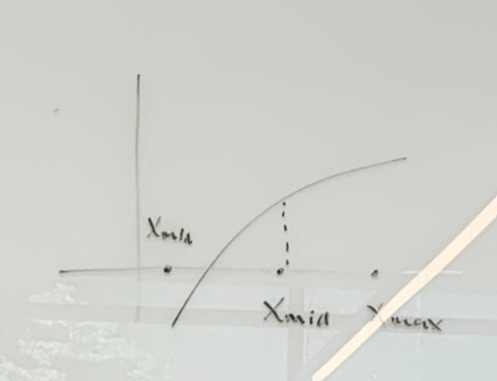
\includegraphics[width = 0.4\linewidth]{Images/410Notes_MATLAB.png}
            
        
    \end{itemize}
    \item After the l-th bisection the width of the search interval is 

    \[ \delta x_l = \delta x_0 2^ {-l} = \frac{x_{max} - x_{min}}{2^l}\]

    This is the upper bound on error in the root estimate

    
\end{itemize}

This is called divide and conquer! 



\newpage
\def \secname {Newton's Method}

\section[\secname]{\hyperlink{toc}{\secname}}


\begin{itemize}
    \item Requires 'good' initial guess $x^{(0)}$, where the number in exponent is the iteration number
    \item 'Good' depends on the problem
    \item One general strategy: $x^{(0)}$ is a solution to a related problem, perhaps with a slightly different parameter, e.g.
\end{itemize}

\textbf{Derivation of Newton's method (Taylor Series)}

Newton's method requires derivative f'(x) pf f(x)

\begin{itemize}
    \item Let $x^*$ be a root of f(x)=0; taylor expand;

    \[0= f(x^*) = f(x^{(n)})+ (x^*-x^{(n)})f'(x^{(n)}) + O((x^* - x^{(n)})^2)\]

    Where $x^n$ is the current estimate

    \[ 0 \approx f(x^{(n)}) + (x^*-x^{(n)})f'(x^{(n)})\]

    Treat as equation; let $x^* \rightarrow x^{(n+1)}$

    \[ 0 \approx f(x^{(n)}) + (x^{(n+1)}-x^{(n)})f'(x^{(n)})\]

    Or

    \begin{equation}
        x^{(n+1)} = x^{(n)} - \frac{f(x^{(n)}}{f'(x^{(n)})}
    \end{equation}

    Where the denominator needs to be not equal to 0


    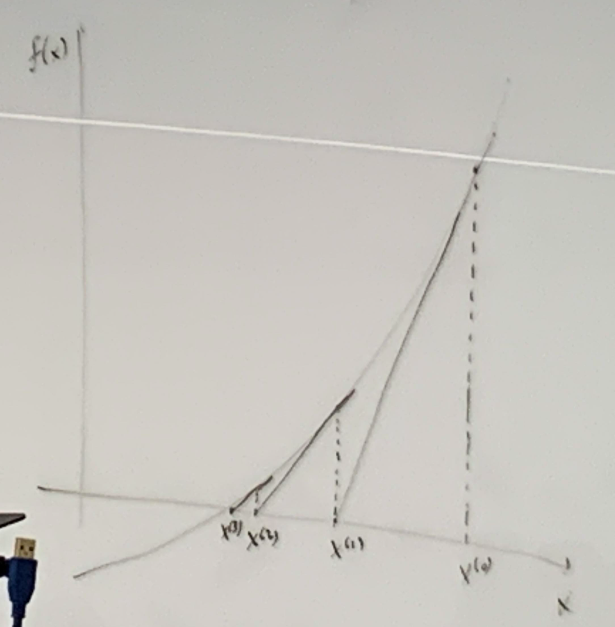
\includegraphics[width = 0.4\linewidth]{Images/410_newtonsmethodinitialguess.png}

    \item Can write iteration as 

    \begin{equation}
        x^{(n+1)} = x^{(n)} - \delta x^{(n)}
    \end{equation}

    \begin{equation}
        f'(x^{(n)}) \delta x^{(n)} = r^{(n)} = f(x^{(n)})
    \end{equation}

    \item Note that we have 

    \[ f'(x^{(n)}) = \frac{f(x^{(n)}}{x^{(n)}-x^{(n+1)}} = \frac{\text{rise}}{\text{run}}\]

\end{itemize}

\textbf{Convergence:} When newton's method converges, does so rapidly, expect number of sig figs to roughly double at each iteration (quadratic convergence).

\vspace{10 px}

\textbf{Example:} "Square Roots"

\begin{equation}
    f(x) = x^2 - a = 0 \qquad \rightarrow \qquad  x^* = \sqrt{a}
\end{equation}

Use other equation

\[ x^{(n+1)} = x^{(n)} - \frac{x^{(n)^2}-a}{2x^{(n)}}\]

\begin{equation}
    \frac{2x^{(n)^2}-(x^{(n)^2}-a)}{2x^{(n)}} = \frac{x^{(n)^2}+a}{2x^{(n)}} = \frac{1}{2} (x^{(n)} + \frac{a}{x^{(n)}}
\end{equation}

\begin{itemize}
    \item Try it with a = 2, 12 digit arithmetic 
    \vspace{10 px}
    Iterate
    \[ x^{(0)} = 1.5\]

    \[ x^{(1)} = \frac{1}{2}(1.5+\frac{2}{1.5}) = 1.416 6666 6667 \qquad \rightarrow \text{3 sig figs}\]

    etc...
\end{itemize}

\subsection{Newton's Method for Systems of equations}

\begin{itemize}
    \item Want to solve
    \[f(x) =0\]

    Where x and f are vectors

    \[x = (x_1 , x_2, ..., x_d)^T\]

    \[ f = (f_1(x), f_2(x),...,f_d(x))^T\]

    Note: Won't always show transpose
    
\end{itemize}

\textbf{Example} (d=2)

\[\sin(xy) = \frac{1}{2}\]

\[ y^2 = 6x+2\]

Ignore fact that we can reduce to d=1 case

Canonical Notation

\[\vec{x}= (x,y)\]

\[ \vec{f} = (f_1(x,y), f_2(x,y))\]

\[ f_1(\vec{x}) = f_1(x,y) = \sin(xy) - \frac{1}{2}\]

\[ f_2(\vec{x}) = f_2(x,y) = y^2 -6x -2 \]

\begin{itemize}
    \item Method again iterate, start from $\vec{x}^{(0)}$

    \item \textbf{Note}: Determining good $x^{(0)}$ more difficult / important than 1-D case;
    Use continuation as necessary
    \item Residual Vector: $\vec{r}^{(n)}$

    \begin{equation}
        \vec{r}^{(n)} = \vec{f}(\vec{x}^{(n)})
    \end{equation}

    \item Analog of f'(x) is Jacobian matric J of first derivatives; elements $J_{ij}$;

    \begin{equation}
        J_{ij} = \frac{\partial f_i}{\partial x_j}
    \end{equation}

    \item Current example

    \[ f_1(x,y) = sin(xy) - \frac{1}{2}\]

    \[ f_2(x,y) = y^2 - 6x -2\]

    \[ \textbf{\underline{\underline{J}}} = \begin{bmatrix}
\frac{\partial f_1}{\partial x} & \frac{\partial f_1}{\partial y} \\

\frac{\partial f_2}{\partial x} & \frac{\partial f_2}{\partial y}
\end{bmatrix} = \begin{bmatrix}
 y \cos{xy} & x\cos{xy} \\
-6 & 2y 
\end{bmatrix}\]
\end{itemize}

\textbf{Newton's Method For Systems of Equations (Continued)}

\begin{itemize}
    \item Derive newton iteration: Multivariate Taylor Series Expansion

    \[ 0 = f(x^*) = f(x^{(n)} + \underline{\underline{J}} [x^{(n)}] \cdot (x^* - x^{(n)} ) + O((x^*-x^{(n)})^2)\]

    Withe Notation: $\underline{\underline{J}} [x^{(n)}] \rightarrow $ Evaluate all Jij's at $x = x^{(n)}$

    \item Drop higher order terms; $x^* \rightarrow x^{(n+1)}$

    \[ 0 = f(x^{(n)} + \underline{\underline{J}} [x^{(n)}] \cdot (x^* - x^{(n)} )\]

    \[ \text{Define } \delta x^{(n)} \equiv - ( x^{(n+1)} - x^{(n)})\]

    \item d-dimensional newton iteration is

    \begin{equation}
        \underline{x}^{(n+1)} = \underline{x}^{(n)} - \underline{\delta x}^{(n)}
    \end{equation}

    Where update vector $\underline{\delta x}^{(n)}$ satisfies dxd linear system

    \begin{equation}
        \underline{\underline{J}}[\underline{x}^{(n)}] \cdot \delta \underline{x}^{(n)} = \underline{f}(\underline{x}^{(n)})
    \end{equation}

    $\rightarrow$ Can be solved in MATLAB using left division operator
    
    \begin{equation}
        J_{ij}[\underline{x}^{(n)}] = \left. \frac{\partial f_i}{\partial x_j} \right|_{\underline{x}=\underline{x}^{(n)}}
    \end{equation}
\end{itemize}

\textbf{General Structure of Newton Solver (PSEUDO CODE HW1!)}

\[x \text{: Solution vector}\]
\[res \text{: Residual vector}\]
\[\underline{\underline{J}} = \text{Jacobian Matrix} \]
\[ dx \text{: Update vector}\]
\[ neq \text{: number of equations}\]

\[ ||v||_2 = rms(v) = \sqrt{\frac{\sum_{i=1}^n v_i^2}{n}} \]


\begin{verbatim}
% x =x^(0)
% while ||dx||_2 > epsilon
%     for i = 1:new
%         res(i) = fi(x)
%         for j = 1:neq
%             J(i,j) = [dfi/dxj](x)
%         end
%     end
%     dx = J \ res % (Linear solve)
%     x = x -dx
% end
\end{verbatim}


\begin{itemize}
    \item Can optimize in MATLAB to not use 2 for loops.

    \item Here and in HW (!!!) should modify above to include code to limit the number of iterations taken (you choose that Number).
    
\end{itemize}

% Missing page

\newpage
\def \secname {Introduction to Finite Difference Approximation (FDA)}

\section[\secname]{\hyperlink{toc}{\secname}}


\subsection{Basic Idea via simple example}
\begin{itemize}
    \item Suppose We are given velocity of particle

    \[ v(t) \equiv \frac{dx}{dt}\]

    \item  Can approximate velocity using 

    \[ v(t) \equiv \frac{dx}{dt} \approx \frac{x(t+\Delta t) - x(t)}{\Delta t}\]

    Some finite increment in time; as $\Delta t \rightarrow 0$, approximation becomes more accurate.

    \item Solve for $x(t+\Delta t)$

    \[ x(t+ \Delta t) \approx x(t) + \Delta t v(t) \]

    \item So, given x(0) can determine

    \[ x(\Delta t) = x(0) + \Delta t v(0)\]
    \[  x(2 \Delta t) =  x(\Delta t) + \Delta t v(\Delta t)\]
    \[  x(3 \Delta t) =  x(2 \Delta t) + \Delta v(2 \Delta t)\] \[...\]

    \item Illustrates 3 key steps in solving ODEs (PDEs) with FDA

    \begin{enumerate}
        \item \textbf{Replace} Continuous Independent variable, t, with discrete values $0,\Delta t, 2\Delta t, 3\Delta t, ...$
        \item \textbf{Discretization of Equations: Replace derivatives with FDAs}
        \item \textbf{Solution:} Solve algebraic equations for approximate solution. Values (Here, once an initial condition x(0) is given)
    \end{enumerate}
\end{itemize}

\subsection{Mathematical Preliminaries}

\subsubsection{Big-O Notation}

\begin{itemize}
    \item Definition: $f(h)$ is $O(h^p)$ (Note: $h$ think stepsize, $\ll 1$) if and only if there are two positive real numbers $M$ , $h_0$ such that 

    \[ |f(h)| \leq M|h^p| \qquad \text{for all } h\ h_0\]

    \[ O(h^2) > O(h^3)\]
\end{itemize}

\subsubsection{Taylor Series}

\begin{itemize}
    \item Taylor series and FDAs
    \begin{itemize}
        \item Can be used to derive FDAs
        \item Can be used to establish accuracy of FDAs (**)
    \end{itemize}
    \item Usually T.S. to expand expressions like $f(x+h)$ (h; expansion parameter) about $f(x)$

    \[ f(x+h) = \sum_{n=0}^\infty h^n \frac{f^{(n)}(x)}{n!} \qquad \text{TS}\]

    for nth derivative of f evaluated at x

    \[ f(x+h) = f(x) + hf'(x) + \frac{1}{2} h^2 f''(x) + \frac{1}{6} h^3 f'''(x) + O(h^4)\]
    \[ f(x-h) = f(x) - hf'(x) + \frac{1}{2} h^2 f''(x) - \frac{1}{6} h^3 f'''(x) + O(h^4)\]    
\end{itemize}

\subsubsection{Discretization: Step 1 : Finite Difference Grids (Meshes, Lattices)}

\begin{itemize}
    \item Physical Domain (Continuum)

    \[ x_{min} \leq x \leq x_{max}\]

    \[ 0 \leq t \leq t_{max}\]
    
    \item Uniform finite difference grid $x_j$

    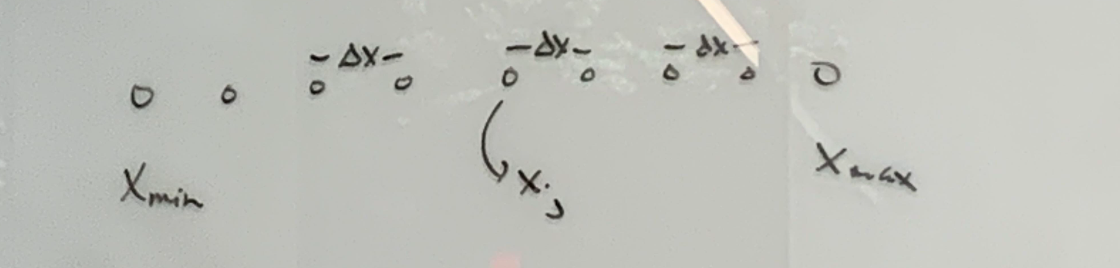
\includegraphics[width = 0.9 \linewidth]{Images/410_discretizationstep.png}


    $\Delta x$ is constant $\rightarrow$ uniform

    \item Grid function notation: $\qquad f(x_j) = f_j$
    \item number of grid points $M_x$

    \item Mesh spacing 

    \[ \Delta x = \frac{x_{max}-x_{min}}{M_x - 1}\]

    Grid points $x_j$

    \[ x_j = x_{min} + (j-1) \Delta x \qquad j = 1,2,...,M_x\]

\end{itemize}

\textbf{Sept 22nd 2023}

\subsubsection{Discretization: Step 2 - derivation of FDAs}

\begin{enumerate}
    \item 3 for first deriv
    \item 1 for 2nd deriv
\end{enumerate}

\begin{itemize}
    \item First, write down, demonstrate accuracy; later derivation
    \item independent variable doesn't matter (use y)
\end{itemize}

\textbf{4.1 First Order, Forward FDA for 1st derivative f'(x)}

\[ f'(x) \approx \frac{f(x+\Delta x)-f(x)}{\Delta X}\]

Note Use a value "forward" of x.

\begin{itemize}
    \item Grid function notation

    \[ f_j' \equiv f'(x_j) \approx \frac{f_{j+1} - f_j}{\Delta x}\]

    \begin{equation}
        f'(x_j) \rightarrow \frac{f_{j+1}-f_j}{\Delta x} \qquad \text{Where the arrow represents "Gets replaced with"}
    \end{equation}

    \item Accuracy?

    \item use taylor series $h\rightarrow\Delta x$ in (TS)

    \[f(x+\Delta x) = f(x) + \Delta x f'(x) + \frac{1}{2} \Delta x^2 f''(x) + \frac{1}{6} \Delta x^3 f'''(x) + O(\Delta x^4) \]

    \item From equation above we have 

    \[ \frac{f(x+\Delta x)-f(x)}{\Delta x} = f'(x) + \frac{1}{2} \Delta x f''(x) + \frac{1}{6} + \Delta x^2 f'''(x) + O(\Delta x^3)\]

    \[ =  f'(x) + \frac{1}{2} \Delta x f''(x) + O(\Delta x^2)\]

    Note: Leading order truncation error is the f''(x) term

    \[ f'(x) + O(\Delta x)\]

    \item Error term $ O(\Delta x) $ means we have first order accurate approx. for the deriv of f(x) at x.

    \item i.e. as $\Delta x \rightarrow 0 $, error in approximation will tend to decrease linearly in $\Delta x$; e.g. as $\Delta x \rightarrow/2 $ we also get error $\rightarrow$ error/2
    
\end{itemize}

\textbf{4.2 First Order Backward FDA for 1st derivative f'(x)}

\[ f'(x) \approx \frac{f(x)-f(x-\Delta x)}{\Delta x}\]

\[ f_j' \equiv f'(x_j) \approx \frac{f_j-f_{j-1}}{\Delta x}\]

\begin{equation}
    f'(x_j) \rightarrow \frac{f_j-f_{j-1}}{\Delta x}
\end{equation}

\begin{itemize}
    \item Accuracy
    \item Again, use Taylor Series

    \[ f(x-\Delta x) = f(x) - \Delta x f'(x) + \frac{\Delta x^2}{2} f''(x) - \frac{\Delta x^3}{6} f'''(x) + O(\Delta x^4)\]

    put equation above into this one

    \[ \frac{f(x)-f(x-\Delta x)}{\Delta x} = f'(x) - \frac{1}{2} \Delta x f''(x) + O(x^2)\]

    \[ = f'(x) + O(x^2)\]
\end{itemize}

\textbf{4.3 Second Order Centred FDA for first derivative f'(x)}

\begin{itemize}
    \item intuitively, taking average of forward, backward should increase accuracy
    \item try:

    \[ \frac{1}{2} \left( \frac{f(x+\Delta x)-f(x)}{\Delta x} + \frac{f(x)-f(x-\Delta x)}{\Delta x} \right)\]

    \[ = \frac{f(x+\Delta x) - f(x-\Delta x)}{2 \Delta x}\]
 
    \begin{equation}
        f'(x_j) \rightarrow \frac{f_{j+1} - f_{j-1}}{2\Delta x}
    \end{equation}
    \item Accuracy

    \[ f(x+\Delta x) = f(x) + \Delta x f'(x) + \frac{1}{2} \Delta x^2 f''(x) + \frac{1}{6} \Delta x^3 f'''(x) + O (\Delta x^4) \]

    \[ f(x-\Delta x) = f(x) - \Delta xf'(x) + \frac{1}{2}\Delta x^2f''(x) - \frac{1}{6} \Delta x^3 f'''(x) + O(\Delta x^4)\]

    Subtract them and lots cancels out

    \[ \frac{f(x+ \Delta x)-f(x-\Delta x)}{2\Delta x} = f'(x) + \frac{1}{6} \Delta x^3 f'''(x) + O(\Delta x^4)\]

    \[ = f'(x) + O(\Delta x^2)\]

    Second order accuracy

    \item  e.g. as $\Delta x \rightarrow \Delta x/2 \qquad \text{we find error} \rightarrow \text{error}/4$

    \item approximation is called "centred"; structure of formula is symmetric about $x_j$
\end{itemize}

\textbf{4.4 Second Order Centred Diff. Approx for f''(x)}

\begin{itemize}
    \item claim: Following is $O(\Delta x^2)$ approx of f''(x)

    \[ f''(x) \approx \frac{f(x+\Delta x) - 2f(x) + f(x-\Delta x)}{\Delta x^2}\]

    \begin{equation}
        f''(x_j) \rightarrow \frac{f_{j+1}-2 f_j + f_{j-1}}{\Delta x^2}
    \end{equation}

    \item Justification: Use Taylor Series

    \[f(x-\Delta x) = f(x) - \Delta x f'(x) + \frac{\Delta x^2}{2} f''(x) - \frac{\Delta x^3}{6} f'''(x) + \frac{\Delta x^4}{24} f''''(x) + O (\Delta x^5)\]

    \[-2f(x) = -2 f(x)\]

    \[ f(x+\Delta x) = f(x) + \Delta x f'(x) + \frac{\Delta x^2}{2} f''(x) + \frac{\Delta x^3}{6} f'''(x) + \frac{\Delta x^4}{24} f''''(x) + O(\Delta x^5)\]

    Subtract terms (reverse engineering style to try to get back to claimed equation)

    \[\frac{f(x+\Delta x) - 2f(x) + f(x-\Delta x)}{\Delta x^2} = f''(x) + \frac{\Delta x^2}{12} f''''(x) + O(\Delta x^4) \]
    \[ = f''(x) + O(\Delta x^2)\]

    Second order error term (as claimed)
    
\end{itemize}


\subsection{Deriving FDAs using taylor series (exam hint)}
\begin{itemize}
    \item Need to choose points that will be used in FDA

    \[ . \qquad . \qquad . \qquad . \qquad . \qquad . \qquad . \qquad . \qquad . \qquad . \qquad . \qquad . \qquad \]

    $x_{j-1}, \qquad x_j, \qquad  x_{j+1}$

    \item Example: Determine approximation to f''(x) that uses $x_j, x_{j+1}, x_{j-1}$

    \item Assume that an appropriate linear combination of truncated taylor series for $f_{j-1}$, $f_j$, $f_{j+1}$ will give the formula 

    \[ \rightarrow \text{consider:} \]
    
    \begin{equation}
        \alpha f_{j-1} + \beta f_j + \gamma f_{j+1} = f''(x) + ...
    \end{equation}

    \item Taylor expanding 

    \[ f_{j-1} = f(x-\Delta x) = f(x) - \Delta xf'(x)+ \frac{1}{2} \Delta x^2 f''(x) - \frac{\Delta x^3}{6} f'''(x) + O(\Delta x^4)\]

    \[ f_j = f(x)\]

    \[ f_{j+1} = f(x+\Delta x) = f(x) + \Delta xf'(x)+ \frac{1}{2} \Delta x^2 f''(x) + \frac{\Delta x^3}{6} f'''(x) + O(\Delta x^4)\]

    \item Now require equation give f''(x) at leading order

    \[ \alpha + \beta + \gamma = 0 \qquad \text{(No f(x) term)}\]
    \[ -\alpha  + \gamma = 0 \qquad \text{(No f'(x) term)}\]
    \[\frac{\Delta x^2}{2}(\alpha + \gamma)=1 \qquad \text{(Gives us f''(x))}\]

    \item Solving

    \[\alpha = \frac{1}{\Delta x^2}\]

    \[ \beta = \frac{-2}{\Delta x^2}\]

    \[ \gamma = \frac{1}{\Delta x^2}\]

    \item So our FDA is 

    \[ f''(x_j) \rightarrow \frac{f_{j+1}-2f_j + f_{j-1}}{\Delta x^2}\]
    
\end{itemize}


problem hint for exam

\subsection{Canonical method for specifying grid spacing (nuts and bolts topic)}

\[ . \qquad . \qquad . \qquad . \qquad . \qquad . \qquad . \qquad . \qquad . \qquad . \qquad . \qquad . \qquad \]

Mesh (partial) grid with each dot separated by $\Delta x$

\vspace{10 px}

Nothing special about spacing, so we can change it if we want...?

\begin{itemize}
    \item Whenever solving DE's with FDA, change $\Delta x$ to see what happens 
    \item Changes by a factor of 2 are most convenient
    \[ \Delta x, \Delta x/2, \Delta x/4, \Delta x/8 ...\]

    \[ l , l+1, l+2, l+3\]

    \item Discretization parameter: Level l

    \[ n_x = 2^l + 1\]

    \[ \Delta x = \frac{x_{max}-x_{min}}{2^l}\]

    Just easier to think/specify in terms of l.

    \item Very small values of l not likely to be of much use; more likely to use $ l = 6,7,8,...$ corresponding to $n_x = 65,129,257,...$

    \item As $l$ and $n_x$ get larger, $\Delta x$ gets smaller and FDA should become more accurate.
\end{itemize}

\subsection{Richardson Extrapolation}
\begin{itemize}
    \item Basic Idea: FD approximation using different scales of discretization $\Delta x_1,\Delta x_2,\Delta x_3,...$ but the same F.D. template $\rightarrow$ combine to get higher order approximation.
    \item Example: Forward approx. of first derivative
    \item Recall

    \[ L^{\Delta x} f = \frac{f(x+\Delta x)+f(x)}{\Delta x} = f'(x) + \frac{1}{2} \Delta x f''(x)+ \frac{1}{6} \Delta x^2 f'''(x) + O(\Delta x^3)\]

    \[ L^{2\Delta x} f = \frac{f(x+2\Delta x)+f(x)}{2\Delta x} = f'(x) + \frac{1}{2} 2\Delta x f''(x)+ \frac{1}{6} 2\Delta x^2 f'''(x) + O(\Delta x^3)\]

    \item Take linear combination

    \[ \alpha L^{\Delta x} f+ \beta l^{2\Delta x} f = f'(x) + O(\Delta x^2)\]

    So giving us

    \[ \alpha + \beta = 1 \]

    \[ \alpha + 2\beta = 0 \]

    ("again this sort of thing is Good for exam purposes again")

    \item Solve 2 equations 

    \[ \alpha = 2\]

    \[ \beta = -1 \]

    giving us

    \[ \alpha L^{\Delta x} f+ \beta l^{2\Delta x} f = s\left( \frac{f_{j+1}-f_j}{\Delta x}\right) - \left(\frac{f_{j+2}-f_j}{2 \Delta x}\right) \]

    

    \[ \rightarrow \qquad \frac{1f_{j+2}+4f_{j+1}-3f_j}{2\Delta x}\]

    \[ = f'(x) - \frac{1}{3} \Delta x^2 f'''(x) + O (\Delta x^3) = f'(x) + O(\Delta x^2)  \]

    \item Can linear combination of 3,4,... approximations to constant even more accurate formulae
    
    
\end{itemize}


\newpage
\def \secname {The Nonlinear Pendulum}

\section[\secname]{\hyperlink{toc}{\secname}}

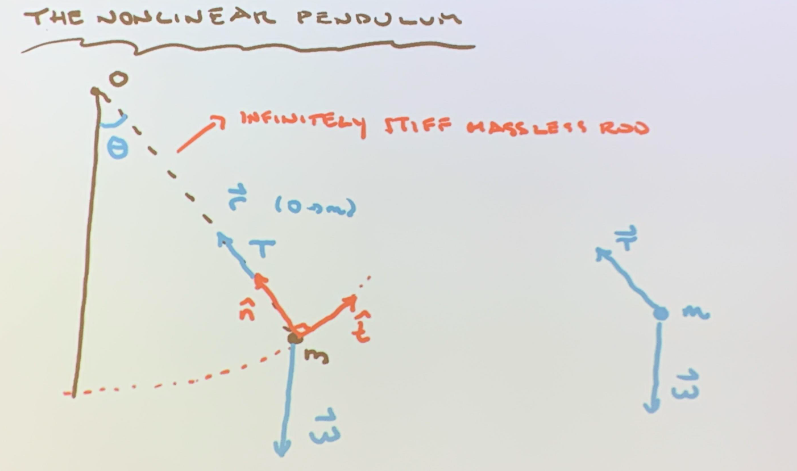
\includegraphics[width = 0.75 \linewidth]{Images/410_pendulumnonlinear.png}

\subsection{Physical and Mathematical Formulation}
\begin{itemize}
    \item Mass of Bob: m
    \item Infinetely rigid, massless pendulum arm; Length L $\equiv |\vec{r}|$
    \item No friction at pivot point. 0
    \item total mechanical energy (kinetic and potential) conserved
\end{itemize}
\subsubsection{Derivation of equation of motion}

\begin{itemize}
    \item Displacement vector $\vec{r}(t)$
    \item $\vec{r}(t)$ makes angle $
    \theta(t)$ (dynamical variable) with vertical
    \item Normal-tangential coordinate system, unit vectors; $\hat{n}$ and $\hat{t}$
    \item Velocity $\vec{v}(t)$ of Bob

    \[ \vec{v}(t) = \frac{d\vec{r}}{dt} = v \hat{t}\]
    \[ v \equiv |\vec{v}|\]

    Velocity is purely tangential
    
    \item Acceleration $\vec{a}(t)$

    \[ \vec{a}(t) = \frac{d^2\vec{r}}{dt^2} = \frac{d\vec{v}}{dt} = \frac{d}{dt} (v\hat{t}) = \frac{dv}{dt} \hat{t} + v \frac{d\hat{t}}{dt} = \frac{dv}{dt} \hat{t} + \frac{v^2}{L} \hat{n}\]

    Using $\frac{d\hat{t}}{dt} = \frac{v}{L} \hat{n}$ and fact that L is constant

    \item no motion in normal direction; consider only tangential motion
    \item tension force $\vec{T} = T \hat{n}$ and normal component of weight wcost irrelevant
    \item newton's 2nd law:

    \[ ma_t = F_t = -\omega \sin \theta = -mg \sin \theta \]

    where g is the acceleration due to gravity

    \[ a_t = -g \sin \theta \]

    \item rewrite as a function for $\theta (t)$

    \item angular velocity

    \[ \omega (t) = \frac{d\theta}{dt}\]

    \item Angular acceleration

    \[ \alpha(t) = \frac{d\omega}{dt} = \frac{d^2\theta}{dt^2}\]

    \[ L \alpha = a_t = L \frac{d^2\theta}{dt^2}\]

    \item sub in equation above and get:

    \[ \frac{d^2\theta}{dt^2} = -\frac{g}{L} \sin\theta \qquad 0 \leq t \leq t_{max}\]

    \item Need initial conditions

    \[ \theta(0) = \theta_0\]
    \[ \omega(0) = \omega_0\]

    these are specified values
\end{itemize}

\subsubsection{Non-dimensionalization}

\begin{itemize}
    \item Can change system of units so g=1, L=1, simplifies equation of motion; using \textbf{Natural Units} for problem.
    \item Adopting our new set of units, we want to solve is:

    \begin{equation}
        \frac{d^2\theta}{dt^2} = - \sin\theta \qquad 0 \leq t \leq t_{max}
    \end{equation}

    with initial conditions

    \begin{equation}
        \theta(0) = \theta_0
    \end{equation}

    \begin{equation}
        \omega(0) = \omega_0
    \end{equation}

    \item Equation above is nonlinear; can solve in closed form but the solution is complicated; FDA solution is no more complicated for a nonlinear case than for a linear case.
\end{itemize}

\subsubsection{Linear Limit}

\begin{itemize}
    \item Assume $\theta(t) \ll 1$

    \[ \sin \theta \approx \theta\]

    (3) $\rightarrow$

    \begin{equation}
        \frac{d^2\theta}{dt^2} = - \theta \qquad 0 \leq t \leq t_{max} 
    \end{equation}

    \item Has clenemal solution

    \[ \theta (t) = A \sin(t + \delta) \]

    where natural units, $\Omega \equiv 1$

    and $A, \delta $ determined by initial conditions

    \[ \Omega \equiv \sqrt{\frac{g}{L}} = 1 \]

    Independent of oscillation amplitude, A (equivalently independent of initial conditions)

    \item Not the case for the nonlinear pendulum
\end{itemize}

\subsection{Solution via FDA}

(HINT: serves as prototype for work in project 1)

Recall method:

\begin{itemize}
    \item Illustrates 3 key steps in solving ODEs (PDEs) with FDA
    \begin{enumerate}
        \item \textbf{Replace} Continuous Independent variable, t, with discrete values $0,\Delta t, 2\Delta t, 3\Delta t, ...$
        \item \textbf{Discretization of Equations: Replace derivatives with FDAs}
        \item \textbf{Solution:} Solve algebraic equations for approximate solution. Values (Here, once an initial condition x(0) is given)
    \end{enumerate}
\end{itemize}

Now Implement:

\subsubsection{Discretization: Step 1 - finite difference grid}

\begin{itemize}


    \item Continuous domain:
    \[ 0 \leq t \leq t_{max}\]

    \item Specify mesh via level parameter, l

    \[ n_t = 2^l + 1 \]

    \[ \Delta t = \frac{t_{max}}{n_t+1} = 2^{-l}t_{max}\]

    \[ t^n = (n-1) \Delta t, \qquad n=1,2,..., n_t\]
\end{itemize}

\subsubsection{Discretization Step 2 - Derivation of FDAs}

\begin{itemize}
    \item Continuum equations $\rightarrow$ Discrete Equations

    \[ \theta^n \equiv \theta (t^n) \equiv \theta ((n-1)\Delta t)\]
    

    \item One derivative to replace, use $O(\Delta t^2)$ centred approximation

    \begin{equation}
        \left. \frac{d^2 \theta}{dt^2} \right|_{t=t^n} \approx \frac{\theta^{n+1}-2\theta^n + \theta^{n-1}}{\Delta t^2}
    \end{equation}

    \begin{itemize}
        \item $t^{n+1}$
        \item $t^n \quad \rightarrow$ Centre-point for formula
        \item $t^{n-1}$
    \end{itemize}

    \item Should evaluate $\sin\theta$ at $t = t^n \quad \rightarrow \sin \theta^n$

    \item substituting in the equation above (27)

    \begin{equation}
        \frac{\theta^{n+1}-2\theta^n + \theta^{n-1}}{\Delta t^2} = -\sin\theta^n \qquad n+1 = 3,4,...,n_t
    \end{equation}
\end{itemize}


\textbf{Nonlinear pendulum (continued) September 29th 2023}

\begin{itemize}
    \item Sove for $\theta^{n+1}$
    \begin{equation}
        \theta^{n+1} = 2\theta ^n - \theta^{n-1} - \Delta t^2 \sin \theta^n \qquad n+1= 3,4,...,n_t
    \end{equation} 

    \item First discrete time we can use this, $t^{n+1} = t^3$

    \item Need value $\theta' = \theta(0)$; $\theta^2 = \theta(\Delta t)$ to initialize scheme 

    \item $\theta ' $ given by initial condition
    \[ \theta ' = \theta (0) = \theta_0\]

    \item $\theta^2 \rightarrow$ bit more involved; state without proof that we need $\theta^2$ to $O(\Delta t^3)$ accuracy so that overall solution is $O(\Delta t^2)$

    \item Heuristic justification: $t=t_{max}$ final time number of time steps is $\approx \frac{1}{\Delta t} = O(\Delta t^{-1})$. So per time step error needs to be $O(\Delta t^3)$ so that overall solution is $O(\Delta t^2)$

    \item Proceed via taylor series, use initial conditions 

    \[ \theta(\Delta t) = \theta (0) + \Delta t \frac{d\theta}{dt}(0) + \frac{1}{2} \Delta t^2 \frac{d^2\theta}{dt^2} (0) + O(\Delta t^3)\]

    \[ \approx \theta_0 + \Delta t \omega_0 + \frac{1}{2} \Delta t^2 \frac{d^2\theta}{dt^2}(0)\]

    Use equation of motion

    \[ = \theta_0 + \Delta t \omega_0 - \frac{1}{2} \Delta t^2 \sin\theta_0\]

    \item Assembling results

    \[ \theta^{n+1} = 2 \theta^n - \theta^{n-1} - \Delta t^2 \sin\theta^n \qquad n+1=3,4,...,n_t\]

    \[ \theta^1 = \theta_0\]

    \[ \theta^2 = \theta_0 + \Delta t \omega_0 - \frac{1}{2} \Delta t^2 \sin\theta_0\]

    \item Now have $n_t$ equations in $n_t$ unknowns and can solve.
\end{itemize}


\subsection{Convergence Analysis (error analysis)}

\begin{itemize}
    \item Want to examine behaviour of solution as $\Delta t \rightarrow 0$

    \item Assumption (Richardson, 1909) Let $U_*(t)$ be the exact (continuum) solution of some differential equation (example the equations above in example); then error is 

    \[ e(t^n) \equiv U_*(t^n) - U(t^n)\]

    Where $U(t^n)$ is the computed value

    \vspace{10px}

    And takes the form 

    \[ \lim_{\Delta t \rightarrow 0} e(t^n) = \Delta t^2 e_2(t^n) + O(\Delta t^4)\]

    where $e_2$ term is some function not some "random" error that would be seen in analyzing experimental data.
    \vspace{10px}
    note that order is 4 because the FDA is centred

    \item How do we know this?

    \item Deep question. Our approach: is to use it as an assumption for convergence analysis.
\end{itemize}

\subsubsection{Convergence Test}

Some mesh:
\[ o \qquad o \qquad o \qquad o \qquad o \qquad o \qquad o \qquad o \qquad o \qquad o \qquad o \qquad \]

\[ l, \Delta t_l, u_l^n\]

\[ o \quad o \quad o \quad o \quad o \quad o \quad o \quad o \quad o \quad o \quad o \quad \]

\[ l+1, \Delta t_{l+1} = \Delta t/2, u_{l+1}^n\]

\[ o \hspace{3 px} o \hspace{3 px} o \hspace{3 px} o \hspace{3 px} o \hspace{3 px} o \hspace{3 px} o \hspace{3 px} o \hspace{3 px} o \hspace{3 px} o \hspace{3 px} o \hspace{3 px} \]

\[ l+2, \Delta t_{l+2} = \Delta t/4, u_{l+2}^n\]

Always use at least 3 grids/ meshes, values of l
\begin{itemize}
    \item Then from equation above we have

    \[ u_l^n \approx u_*^n - (\Delta t_l)^2 e_2^n\]

    \[ u^n_{l+1} \approx u_*^n - (\Delta t_{l+1})^2 e_2^n\]

    \[ u^n_{l+2} \approx u_*^n - (\Delta t_{l+2})^2 e_2^n\]

    Think of n labelling common set of times (times on caorse gride l)

    \item Now subtract solutions on adjacent levels 

    \[ u_l^n-u_{l+1}^n \approx -((\Delta t_l)^2 - (\Delta t_{l+1})^2)e_2^n = \frac{-3}{4} \Delta t_l^2 e^n_2\]

     \[ u_{l+1}^n-u_{l+2}^n \approx - \frac{3}{4}((\Delta t_{l+1})^2 e_2^n = \frac{-3}{16} \Delta t^2_l e^n_2\]

     where the last term is error reduced by factor of 4

     \item Observation 

     \begin{enumerate}
         \item Get estimate of solution error by simply subtracting solutions on adjacent levels

         From equation earlier we have 

         \[ e^n = \Delta t^2 e_2^n + ...\]

         \[ u_l^n - u^n_{l+1} \approx -\frac{3}{4} (\Delta t_l)^2 l^n_2\]

         so 

         \[ -\frac{4}{3} (u_{l}^n - u_{l+1}^n) \approx e^n\]

         \item Consider the ratio

         \[ \frac{u^n_l - u^n_{l+1}}{u^n_{l+1} - u^n_{l+2}}\]

         in limit that $\Delta t_l \rightarrow 0$ should  get 

         \[ \frac{-(3/4)(\Delta t_l)^2 e_2^n}{-(3/16)(\Delta t_l)^2 e^n_2} = 4\]

         \item More useful in practice: scale (multiply) differences

         \[ u_l^n - u_{l+1}^n\ \text{by } 4^0=1\]
         \[ u_{l+1}^n - u_{l+2}^n\ \text{by } 4^1=4\]
         \[ u_{l+2}^n - u_{l+3}^n\ \text{by } 4^2=16\]

         And plot them (as a function of $t^n$) on single graph

         \vspace{10px}

         Curves should be nearly coincident and agreement should get better for higher levels

         \item Can use as many levels in the test as is feasible but use a minimum of 3

         \item \underline{Important}: don't have to know what the error is to do a convergence test

         \item \underline{Important}: If we don't observe convergence, good indication that we need to do some debugging.
     \end{enumerate}

\end{itemize}


\textbf{11:10am October 4th 2023}

\textbf{Energy Conservation}

Mechanical energy is conserved = use as check on implementation

\begin{itemize}

    \item For nonlinear pendulum

        \[ \text{kinetic energy} \equiv T(t) = \frac{1}{2} mv(t)^2 = \frac{1}{2} m (L \omega (t))^2\]

        \[ \text{potential energy} \equiv V(t) = mgh(t)\]

        where h(t) is vertical displacement of bob from equilibrium height

        \[ \text{total energy} = E(t) = T(t) + V(t)\]

        
    \[ \text{Total Energy } = E(t) = T(t) + V(t) \]

    \[ E(t) = \frac{1}{2} m (L\omega(t))^2 + mgL(1-\cos\theta(t))\]

    
    \item Our units: g=1, L=1, m=1 (MLT)

    \[ E(t) = T(t) + v(t) = \frac{1}{2} \omega (t)^2 + (1-\cos\theta(t)\]

    \item Track deviation in energy 
    \[ dE(t) \equiv E(t)-E(0)\]

    \item One thing to do: plot it and see whether it "Looks Good"

    \item Better: Check convergence of $dE(t;\Delta t)$

    \[ \Rightarrow \text{Expect} \qquad dE(t; \Delta t) = \Delta t^2 \epsilon(t) + ... \qquad \text{Where epsilon is some function}\]

    \[ \Rightarrow \text{As } \Delta t \rightarrow 0 \qquad dE(t;\Delta t) \rightarrow 0 \text{ As } \Delta t^2\]

    \[ \Rightarrow \text{Plot } \quad dE(t; \Delta t), 4dE(t; \Delta t/2), 16 dE(t; \Delta t/4), ...\]

    Should be neatly coincident

    \item Calculations should display convergence to conservation

    \item For \textbf{linear} pendulum need another expression for total energy
    \item Small angle approximation

    \[ \cos\theta = 1 - \frac{1}{2} \theta ^2 + O(\theta^4) \approx 1- \frac{1}{2}\theta^2\]

    \[ \Rightarrow E_{Linear}(t) = T(t) + V(t) = \frac{1}{2}\omega(t)^2 + \frac{1}{2} \theta (t)^2\]
    
\end{itemize}

\textbf{End of FDA discussion - will use convergence testing and FDA lots in projects and HW!}


\newpage
\def \secname {Solving Ordinary Differential Equations (ODEs)}

\section[\secname]{\hyperlink{toc}{\secname}}


\subsection{Casting Systems  of ODEs in first-order form}

\begin{itemize}
    \item Can always reduce a system of ODEs to a set of first order DEs by introducing appropriate new (auxiliary) variables
    \vspace{10px}
    Example 1:

    \begin{equation}
        y''(x) + q(x) y'(x) = r(x) \qquad '\equiv \frac{d}{dx}
    \end{equation}

    This is second order since the highest derivative is ''

    \item Introduce new variable $z(x) \equiv g'(x) $ then (30) becomes 

    \[ y' = z\]

    \[ z' = r-qz\]

    No derivatives on the RHS

    \vspace{10px}
    Example 2:

    \begin{equation}
        y''''(x) = f(x)
    \end{equation}

    \item Introduce new variables

    \[ y_1 (x) \equiv y'(x)\]
    \[ y_2 (x) \equiv y''(x)\]
    \[ y_3 (x) \equiv y'''(x)\]

    Then (31) Becomes;

    \[ y'=y_1\]
    \[ y_1'=y_2\]
    \[ y_2'=y_3\]
    \[ y_3'= f\]

    \item Thus, generic problem in ODEs is reduced to study of N coupled, \textbf{first order} DEs for functions 

    \[y_i = 1,2,3,... N\]

    \begin{equation}
        y_i'(x) \equiv \frac{dy_i}{dx} (x) = f_i(x,y_1,y_2,...,y_N) \qquad i = 1,2,.., N
    \end{equation}

    Where the $f_i$ are known functions of $x$, $y_i$

    Equivalent forms

    \[\underline{y}'(x) = \underline{f}(x,y)\]

    \[ \underline{\dot{y}}(t) = \underline{f}(t,\underline{y})\]

    dot is the time derivative 
\end{itemize}

Now to actually solve some ODEs we need something else...

\subsection{Boundary/ Initial Conditions}

\begin{itemize}
    \item ODE problem not completely specified by ODEs themselves
    \item Generally, boundary conditions (BCs) are algebraic conditions on the yi in (32) that are to be setastifed at discrete specified points.

    \item Nth order system $\Rightarrow$ need N conditions

    \item BCs divide ODE problems into 2 broad classes:

    
    \begin{enumerate}
        \item Initial value problem
        \item Boundary value problem
    \end{enumerate}
    
    \subsubsection{Initial Value Problems}
    
    \begin{itemize}
        \item  All the $y_i$ are given at some initial value $t_{min}$ (0), wish to find the $y_i$ at some final value $t_{max}$ (or set of values)

        \[ t_n \qquad t_{min} \leq t_n \leq t_{max} \quad n=1,2,...\]

        \item Most relevant for recasting of ODEs in first order form
    \end{itemize}

    \subsubsection{(Two Point) Boundary Value Problems}

    \begin{itemize}
        \item BC's Specified at more than one value of x; 

        typically: some at $x_{min}$, some at $x_{max}$
    \end{itemize}
\end{itemize}

\subsection{Solution of ODEs (Initial Value Problems): Basic Methods}

\subsubsection{Euler Methods}

\begin{itemize}
    \item Consider the basic ODE
    \[ y'(x) = f(x,y)\]

    To be solved on some interval $[x_0, x]$ where $y(x_0)$ is given.
    \item One approach: taylor series

    \[ y(x) = y(x_0) + (x-x_0) y'(x_0) + \frac{(x-x_0)^2}{2} y''(x_0) + \ldots\]

    Where $y'(x_0)=f(x_0,y_0)$
    \item Higher derivatives get messy

    \begin{equation*}
    \begin{aligned}
    y''(x) & = \frac{\partial}{\partial x} f(x,y) + \frac{dy}{dx} \frac{\partial }{\partial y} f(x,y) \\
    & = \frac{\partial f}{\partial x} + f(x,y) \frac{\partial}{\partial y} f(x,y) 
    \end{aligned}
    \end{equation*}
    
    \item Algebraically complicated to go to high order; not \textbf{often} used in practice; good for derivations

    \item Truncate expansion at $O(x-x_0)$
    \[ y(x) \approx y(x_0) + (x-x_0) y'(x_0)\]

    \[ = y(x_0)+(x-x_0)f(x_0,y_0)\]

    where the dx term is equiv to h, i.e. the step size

    \item $\Rightarrow$ Euler Method (forward Euler)

    \begin{equation}
        y(x_0+h) = y(x_0)+h f(x_0, y_0) = y_0 + h f_0
    \end{equation}

    \item Basic algorithm for any ODE integrator: take repeated steps, possibly adjusting step size until integration limit is reached.

    \[ y_{n+1} = y_n + h f_n\]

    \item Accuracy? O(h)

    \item Not recommended for production work

    \item Improve accuracy by using value of y' at mid point of the interval

    \item Want an estimate of $f(x_0+h/2, y(x_0+h/2))$

    \item Compute

    \[ y(x_{mid}) = y_0 + \frac{h}{2} y_0' = y_0 + \frac{h}{2} f_0\]

    \item Modified Euler's method

    \[ y(x_0+h) = y_0+h f(x_{mid}, y_{mid})\]
    \[ x_{mid} = x_0 + \frac{h}{2}\]
    \[ y_{mid} = y_0 + \frac{h}{2} f_0\]

    this is $O(h^2)$ accurate

    \item Improved Euler Method

    \[ y(x_0+h) = y(x_0) + h f_0 + \frac{f(x_0+h, y_0+hf_0)}{2}\]

    Still $O(h^2)$ accurate

    \subsubsection{Improving Euler Methods}

    \begin{itemize}
        \item Taylor Series: use more terms in expansion
        \item Linear Multi-step methods: use data from previous time steps to cancel terms in truncation error
        \item Runge-Kutta methods: use intermediate points within time step

        \item So far we have been looking at:

        \[ y'(x) = f(x,y(x))\]

        \item All methods so far and to come generalize immediately to 

        \[ y_i'(x) = \frac{dy_i}{dx}(x) = f_i(x,y,\ldots, y_N)\]

        for $i=1,2, \ldots, N$

        \[ \mathbf{y}'(\mathbf{x} = \mathbf{f}(x, \mathbf{y}(\mathbf{x}))\]
    \end{itemize}
\end{itemize}

\subsubsection{Runge Kutta Methods}

\begin{itemize}
    \item Modified Euler Methods is an example of a runge-kutta (RK) method of order 2
    \item For any given order, infinite number of distinct RK methods
    \item Very popular example: Fourth order (RK4):

    \[ f_0 = f(x_0, y_0)\]
    \[ f_1 = f(x_0+\frac{h}{2}, y_0+\frac{h}{2}f_0)\]
    \[ f_2 = f(x_0+\frac{h}{2}, y_0+\frac{h}{2}f_1)\]
    \[ f_3 = f(x_0+h, y_0+\frac{h}{2}f_2)\]

    \[y(x_0+h) = y(x_0)+ \frac{h}{6} (f_0 + 2 f_1 + 2 f_2 += f_3)\]

    Here we get $O(h^4)$ accuracy! Good compromise between accuracy and the number of function evaluations.

    \item Non-trivial to derive RK4, but for the case where $f=f(x)$ , can construct it by approximating 

    \[ y(x_0+h) = y(x_0) + \int_{x_0}^{x_0+h} f(x) dx\]

    Integral using Simpson's rule
\end{itemize}

\subsubsection{Adaptive Stepsizes}

\begin{itemize}
    \item In general, want solution of ODEs to some prescribed accuracy

    \item What affects the solution accuracy?

    \begin{itemize}
        \item Step size, h
        \item Accuracy order of method (p)
    \end{itemize}

    \item How do we \textbf{estimate} the solution accuracy?

    \begin{itemize}
        \item Typically estimate \textbf{local} accuracy 
        \item Basic tool: compute solution at $x=x_0+h$ using two different step sizes or methods of different accuracy and then compare them. (HW2 Hint)
    \end{itemize}

    \item How do we control solution accuracy?
    \begin{itemize}
        \item If difference is less than error criterion, accept solution and advance to next time step; otherwise decrease stepsize and repeat integration
        \item If difference is much less than error criterion, increase step size
        \item In practice implement limiters so that stepsizes don't change too much from one time step to another.
    \end{itemize}
\end{itemize}

\subsubsection{Error Control with dual order method}

\begin{itemize}
    \item Two methods (RK, say) with orders of accuracy p, p+1
    \item To leading order, after one step with each method 
    \[ y(x_0+h) = y_{\text{exact}} + k h^{p+1}\]

    p+1 comes from the fact that this is a local error; $O(h^{-1})$ steps to get to any finite time

    \[ \Tilde{y}(x_0+h) = y_{\text{exact}} + \Tilde{k} h^{p+2}\]

    \item Assume h is small; difference between two is

    \[ y(x_0+h) - \Tilde{y}(x_0+h) \approx kh^{p+1} - \Tilde{k}h^{p+2} \approx k h^{p+1}\]

    $\Rightarrow$ direct estimate of the solution error

    \item Typical integrator will use 2 types of error control parameterized by $\epsilon_{\text{ABS}}$, $\epsilon_{\text{REL}}$

    \begin{itemize}
        \item $\epsilon_{\text{ABS}}$: Absolute error control; integrator tries to keep error estimate at/below $\epsilon_{\text{ABS}}$
        \item $\epsilon_{\text{REL}}$: Relative error control; integrator attempts to maintain
        \[\frac{e_{\text{EST}}}{|y(x_0+h)|} \le \epsilon_{\text{REL}}\]
    \end{itemize}

    \item Absolute control: Good when values are O(1) or relatively constant in magnitude or near 0 (numerically ill-conditioned process)

    \item Relative control: good when solution magnitudes vary appreciably 

    \item Can combine two; for example we can say

    \[ e_{\text{EST}} \le \epsilon_{\text{ABS}} + \epsilon_{\text{REL}} |y(x_0+h)|\]

    or \[ e_{\text{EST}} \le \text{MAX}(\epsilon_{\text{ABS}}\text{, } \epsilon_{\text{REL}} |y(x_0+h)|\]

    This is what MATLAB integrators tend to use
\end{itemize}

\subsection{Checking/ Validating results from ODE integrators}

\subsubsection{Monitoring conserved quantities}
\begin{itemize}
    \item Example: for dynamical systems with a Lagrangian/ Hamiltonian, total energy E(t) is conserved

    \item Monitor variation $\delta \hat{E} (t;\epsilon)$ on a solution domain $0 \le t \le t_{max}$

    \[ \delta \hat{E}(t;\epsilon) = \hat{E}(t;\epsilon)-\hat{E}(0;\epsilon)\]

    where $\epsilon \equiv $ error tolerance for integrator 

    \item Should find that $\delta \hat{E}(t;\epsilon)$ is $O(\epsilon)$ 

    \[ \delta\hat{E}(t;\epsilon) = \epsilon g(t) + \ldots\]

    where g(t) is some function

    \item Thus, e.g., if we take $\epsilon\rightarrow\epsilon/10$ should see $\delta \hat{E} \rightarrow\delta\hat{E}/10 $ (approx so long as $\epsilon \gg \epsilon_{\text{machine}}$)
    
\end{itemize}

\subsubsection{Independent residual evaluation}

\begin{itemize}
    \item \textbf{Idea}: Attempt to directly verify that approximate solution (previously y) satisfies the ODEs through the use of an independent discretization of the ODEs (distinct from the one used by the ODE integrator)

    \item Residual $\Rightarrow$ something that should tend to 0 in appropriate limit

    \item Let 

    \[ L[u(t)] \equiv Lu(t) = 0 \]

    where L is a differential operator 

    \begin{itemize}
        \item u(t) can be vector of dependent variables 
        \item most general ODE system 
        \item Assume L linear, but only for convenience
    \end{itemize}

    \item Let $\hat{u}(t;\epsilon)$ be solution computed by ODE integrator at times 

    \[ t^{h} \equiv t_n = t_{min}, t_{min}+h, t_{min}+2h, \ldots, t_{max} \]

    \item Consider second-order centred FDA of $Lu=0$

    \[ L^h u^h = 0\]

    \begin{equation}
        L^h = L + h^2E_2 + O(h^4)
    \end{equation}

    Where E is higher order differential operator (higher than L)

    \item Note that this equation (34) defines $u^h$ and that

    \[ u^h(t) \neq \hat{u}(t^h;\epsilon)\]

    where the u hat term is ODE, integrator

    \item Again, $L^{h}$ can be expanded
    \[ L^h = L + h^2 E_2 + h^4 E_4+ \ldots \]

    Where the E terms are higher order differential operators

    \item Can write

    \[ \hat{u}(t;\epsilon) = u(t) + e(t; \epsilon)\]

    Error in computed solution from ODE integrator

    \item Consider action of $L^h$ on $\hat{u}(t;\epsilon)$

    \[ L^h \hat{u}(\epsilon) = (L+h^2E_2 +h^4E_4+ \ldots ) 
 (u+e(t))\]

    \[ = \cancelto{0}{Lu} + h^2 E_2 u + \ldots L^h e(t)\]
    
    where the last term is small compared to other term


    \[ \Rightarrow L^h \hat{u} \approx h^2 E_2 u = h^2r = O(h^2) \]

    where r is some function

    \[ \text{Assuming \quad } h^2 E_2 \gg L^h e(t)\]

    \item Makeup Monday October 12th 2023

    \item With high accuracy ODE solver is usually possible to satisfy this equation, at least over some time interval $(t_{min}, t_{max})$ and as long as $h$ isn't too small.

    \item KEY idea is to show/check \textbf{correctness} of implementation; e.g. checking for errors in coding of equations
\end{itemize}

\subsubsection{Simple Harmonic Motion Example}

\begin{itemize}
    \item Governing D.E. (unit angular frequency; 0 phase)

    \begin{equation}
        \frac{d^2y(t)}{dt^2} = -y
    \end{equation} 

    \item first order form; define

    \[ y_1(t) \equiv y(t) \qquad y_2(t)\equiv \frac{dy_1}{dt}\]
    \item Then Equation of motion becomes system 

    \[ \frac{dy_1}{dt} = y_2 \qquad \frac{dy_2}{dt} = -y_1\]

    Subject to initial conditions

    \[ y_1(0) = y(0) \qquad y_2(0) = \frac{dy}{dt}(0)\]
\end{itemize}

\textbf{Independant Residual Evaluation}

\begin{itemize}
    \item First rewrite (7) as 

    \begin{equation}
        \frac{d^2y(t)}{dt^2} + y(t) = 0
    \end{equation}

    \item Now, use ODE integrator to generate solution $\hat{u}(t^h;\epsilon)$ on a level-l uniform mesh

    \[ t^h_n = 0,h,2h,\ldots, t_{max}\]

    with 

    \[h=\frac{t_{max}}{2^l}\]

    \item Then apply $O(h^2)$ FDA of equation (36) to $\hat{y}$ to compute residual $R_n$

    \[ R_n \equiv \frac{\hat{y}_{n+1}-2\hat{y}_n+\hat{y}_{n+1}}{h^2} + \hat{y}_n \qquad n=2,3,\ldots , 2^l-1\]

    \item Should find that

    \[ \text{RMS}(R_n) = O(h^2)\]

    \item In particular, compute $R_n$ on 3 separate levels of discretization

    \[ h_1 = h_e\]
    \[ h_2 = 2h_1 = h_{l-1}\]
    \[ h_3 = 4h_1 = h_{l-2}\]

    But using single level-l calculation using the ODE integrator

    \item Then by Plotting 

    \[ 16R^l, \quad 4R^{l-1}, \quad R^{l-1}\]

    On a single graph, should see near-coincidence of the curves $\Rightarrow$ convergence of independent residual.
    
\end{itemize}

\subsection{Passing Additional Arguments to the Derivatives Function}

\begin{itemize}
    \item Systems of ODE often have additional parameters (Change from solution to solution)
    \item The calling sequence for the derivatives function is fixed

    \[ \text{function derivative } = \text{odefun}(t,y)\]

    \item Need mechanism to pass in additional information
    \item At least 3 ways

    \subsubsection{Use an anonymous function definition}

    \begin{itemize}
        \item Example: 3 Parameter a,b,c
        \begin{verbatim}
        code function    odefun(t,y,a,b,c)
        a=1.0
        b = 2.5
        c =3.14
        [tout yout] = ode45(@(t,y) odefun(t,y,a,b,c, ... tspan, yphi)
        \end{verbatim}
    \end{itemize}

    \subsubsection{Use a Global Variable}
    \begin{itemize}
        \item Be default, scope of matlab variable is local to programming unit (Script, function)
        \item Change this behaviour by using global command
        \item Must use declaration in all programming units in which we want access to variable

        \begin{verbatim}
            % Script; function-caller
                .
                .
                .
            global m;
            m = 1.56;
                .   
                .
                .
            [you yout] = ode45(@fcn, [0.0 1.0], [0.0 2.0]);
                .
                .
                .
            function derivs = fcn(t,y)
                global m;
                    .
                    .
                    .
            end
        \end{verbatim}

        \item Syntax for multiple global variables:

        \begin{verbatim}
            global a b c;
        \end{verbatim}

        Note: no commas
    \end{itemize}

    \subsubsection{Adjoin parameter to ODE system}

    \begin{itemize}
        \item Treat any parameter as a \textbf{dependent} variable with a trivial governing ode
        \item for example 
        \[ \frac{dm}{dt} = 0 \qquad m(0) = 1.56 \Rightarrow m=\text{const} = 1.56\]

        \item A bit more computationally intensive than the other two approaches; and a bit more complicated to implement.


        $\Rightarrow$ (Matt) Advocates using anonymous functions (although he uses global variables).
    \end{itemize}

    \item See example of dumbbell orbit slides from the course site
\end{itemize}

\subsection{The one dimensional Toda Lattice}

(following https://www.mat.univie.ac.at/~gerald/ftp/book-jac/toda.html)\newline

Model for crystal (simple solution), particle sites with spring between sites:

\[ . \quad . \quad . \quad . \quad . \quad . \quad . \quad . \quad . \quad . \quad . \quad . \quad .\]

with nearest neighbour interactions

\begin{itemize}
    \item Let g(n,t) be displacement of particle n from its equilibrium position; p(n,t) its momentum (m=1) and V(r) the interaction potential where r is the interparticles separation.

    \item Hamiltonian

    \[ \mathcal{H} (p,q) = \sum_n \frac{p(n,t)^2}{2} + V(q(n+1,t)-q(n,t))\]

    \item Example: Harmonic Interaction

    \[ V(r) = r^2\]

    \item Resulting set of equations are linear, with constant set of coefficients

    \item Solution: super position of normal modes

    \item \textbf{Solitons}: pulse like waves which propagate and interact similarly to particles
    \item \textbf{Nonlinear}: Dispersion balances non linearity (Focusing)
    \item Motivation in part by soliton theory, TODA (1967) came up with a potential 

    \[ V(r) = e^{-r} + r-1\]

    where the r-1 term means we get harmonic behaviour in small r limit

    \item Equations of Motion:

    \[ \frac{d}{dt} p(n,t) = e^{-(q(n,t)-q(n-1,t))}-e^{-(q(n+1,t)-q(n-1,t))}\]

    \[ \frac{d}{dt} q(n,t) = p(n,t) \qquad n=1,2,\ldots, n_{sites}\]

    \item Can show that the following is a solution

    \[ q_1(n,t) = q_+ + \log (\frac{N}{D}\]

    \[ N = 1+ \frac{\gamma}{1-e^{-2\kappa}} \text{exp}(-2\kappa n + 2 \sigma \sinh (k) t)\]

    \[ D = N \qquad \text{BUT} \qquad n\rightarrow n+1\]

    \item Can put some example values in like
    \[ \kappa = \gamma  = q_+ = 1.0 \qquad \text{and} \quad \sigma = 1\]
    and we get a "kink" solution (looks like heaviside function sorta)

    \item Propogrates to the right is sigma is +1 and left if sigma is -1

    \item Speed of propagation is $\sinh(\kappa)/\kappa \Rightarrow$

    Thinner kinks travel with higher speeds

    \item Refer to Slide on Course Site for ODE MATLAB Implementation of this Toda Lattice Problem
\end{itemize}


\textbf{October 18th 11:07am}

\textbf{THE VAN DER POL OSCILLATOR }\newline 


(following Tsatsos ...)

\begin{itemize}
    \item 1920s Van der Pol (VdP) experimented with oscillations in a vacuum tube triode circuit
    \item Concluded that all initial conditions converged to some finite-amplitude periodic category
    \item Proposed a non-linear ODE to model phenomena
    \item (unforced VdP equation)
    \begin{equation}
        \frac{d^2x}{dt^2}+ a(x^2-1) \frac{dx}{dt} + x = 0
    \end{equation}
    Where a is constant (parameter) and when a=0 we get linear oscillator

    \item Version of equation 37 here that includes forcing term

    \[ \frac{d^2x}{dt^2} + a(x^2-1) \frac{dx}{dt} + x = b s\sin(\omega t)\]

    where $b$ and $\omega$ are parameters (constants)

    \item Model has application in: physics, electronics, biology, neurology, sociology, economics
    \item view VdP equation as "typical" nonlinear dynamical system; illustrates some of qualitative ways we can describe such systems
\end{itemize}

\subsubsection{Analysis Methods}
\begin{enumerate}
    \item \textbf{Phase Space Plots}: Good for 2-D systems (one x, one p (dx/dt); plotting trajectories in phase space $\Rightarrow$ reveal nature of dynamics

    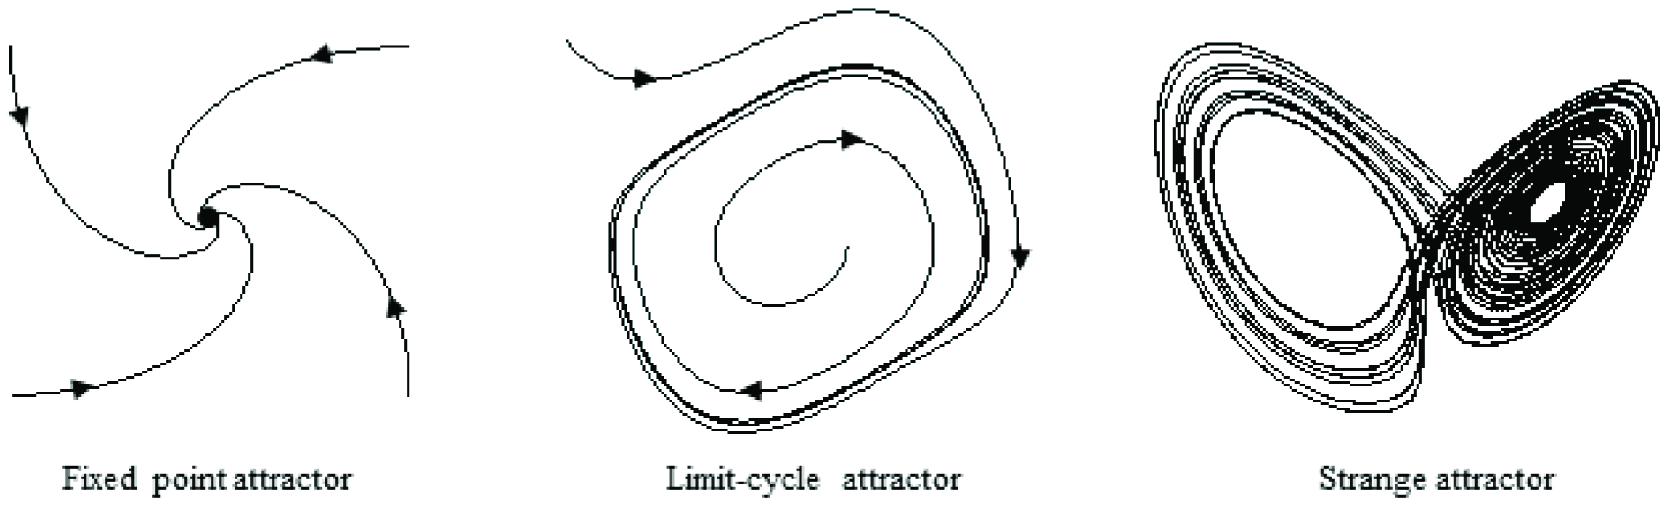
\includegraphics[width = \linewidth]{Images/attractor_types.png}
    

    \item Nature of long-time attractors

    \begin{enumerate}
        \item \textbf{Fixed Point:} trajectory converges to a single point in phase space
        
        \item \textbf{Limit Cycle}: (Periodic Trajectories) Trajectory converges to closed curve in phase space (undamped oscillator)
        
        \item \textbf{Strange Attractor}: Trajectory converges to "curve" with fractional dimension in phase space \newline 

        Coastline structure on all scales 

        \[ l \approx x^{(d-1)} \qquad 1 \le d \le 2 \]
        
    \end{enumerate}

    \item \textbf{Poincare Section:} view dynamics periodically sometimes projecting onto a space with reduced dimensionality (1d on 2d typically) for case of driven dynamics, natural period is period of forcing. Resulting trace of dynamics is called Poincare section. Various features can appear

    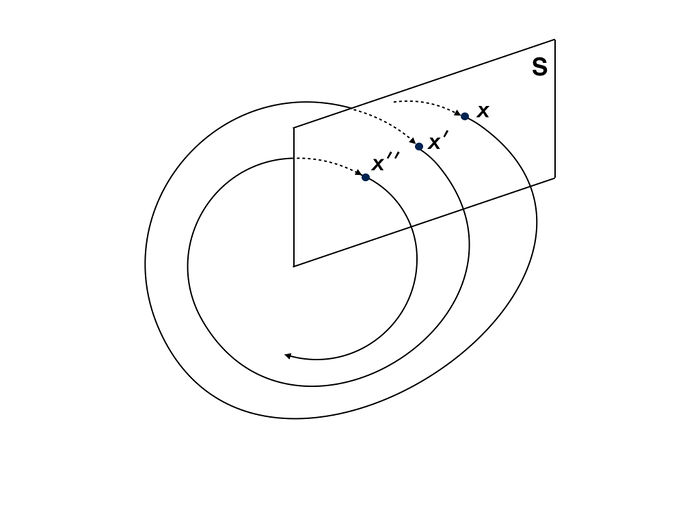
\includegraphics[width = \linewidth]{Images/poincare_section.jpg}

    \begin{enumerate}
        \item Fixed Points: single points on Poincare section
        \item Limit Cycles: will appear as one or more isolated points
        \item Almost periodic trajectory: will appear as a near-continuous curve
        \item Chaotic dynamics: will appear as a "curve" with fractional dimensions
    \end{enumerate}
    \item Bifurcation Diagram \newline
    
    Plots which show dependence of Poincare section on a problem parameter typically, plot a certain number of points in a given Poincare section, as a function of the parameter \newline 

    Typical use here; show transition to chaos (period doubling for example)

    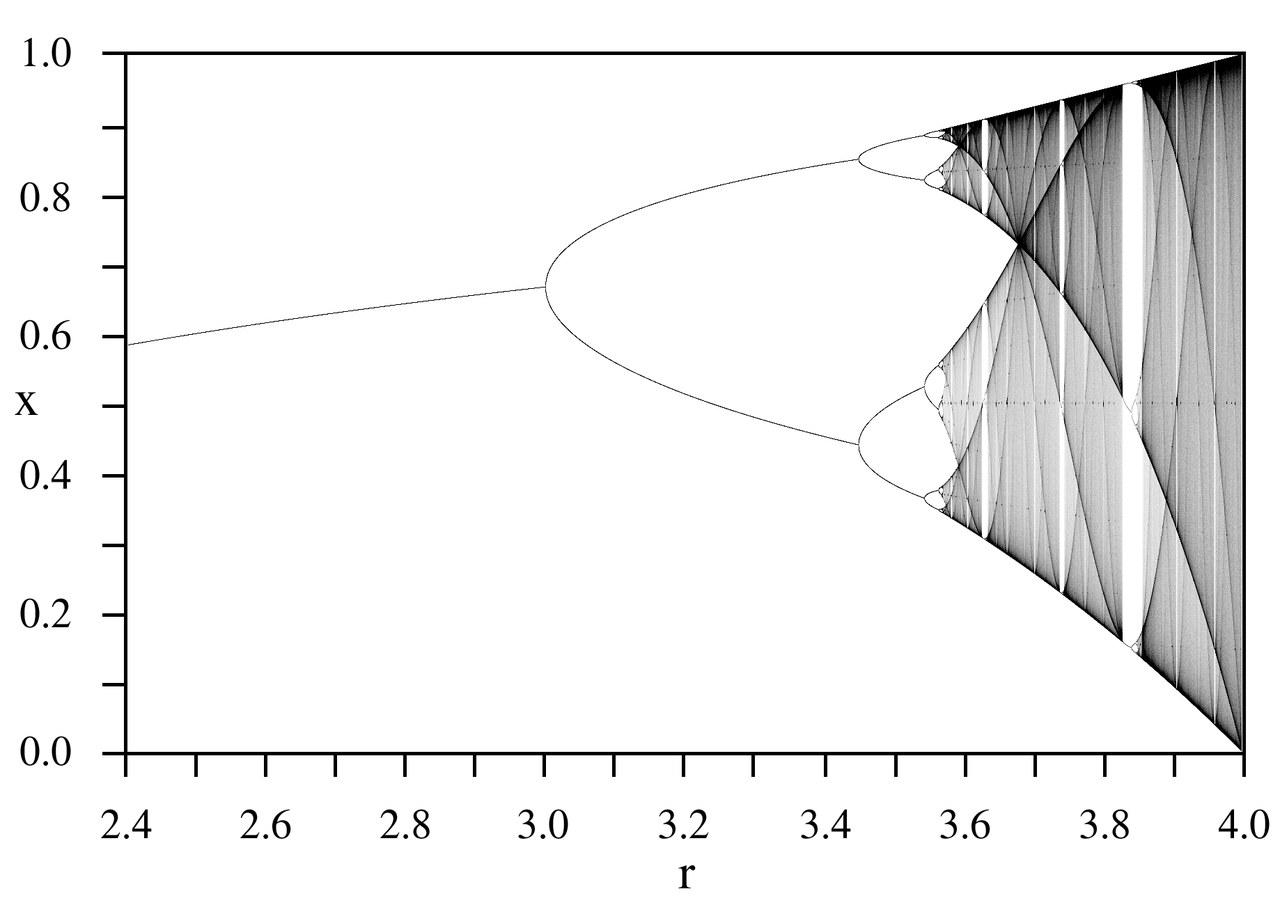
\includegraphics[width = \linewidth]{Images/bifurcation_diagram.png}
\end{enumerate}

\textbf{October 20th 2023, 11:00am}

\subsection{Boundary Value Problems - Shooting}

\begin{enumerate}
    \item Introduction \newline
\end{enumerate}

Recall: 2-PT Boundary value problems; B.C.'s supplied at two points - typically end points of the solution domain
\begin{itemize}
    \item In idealized physical problems, one of the points will often be $x = \infty$

    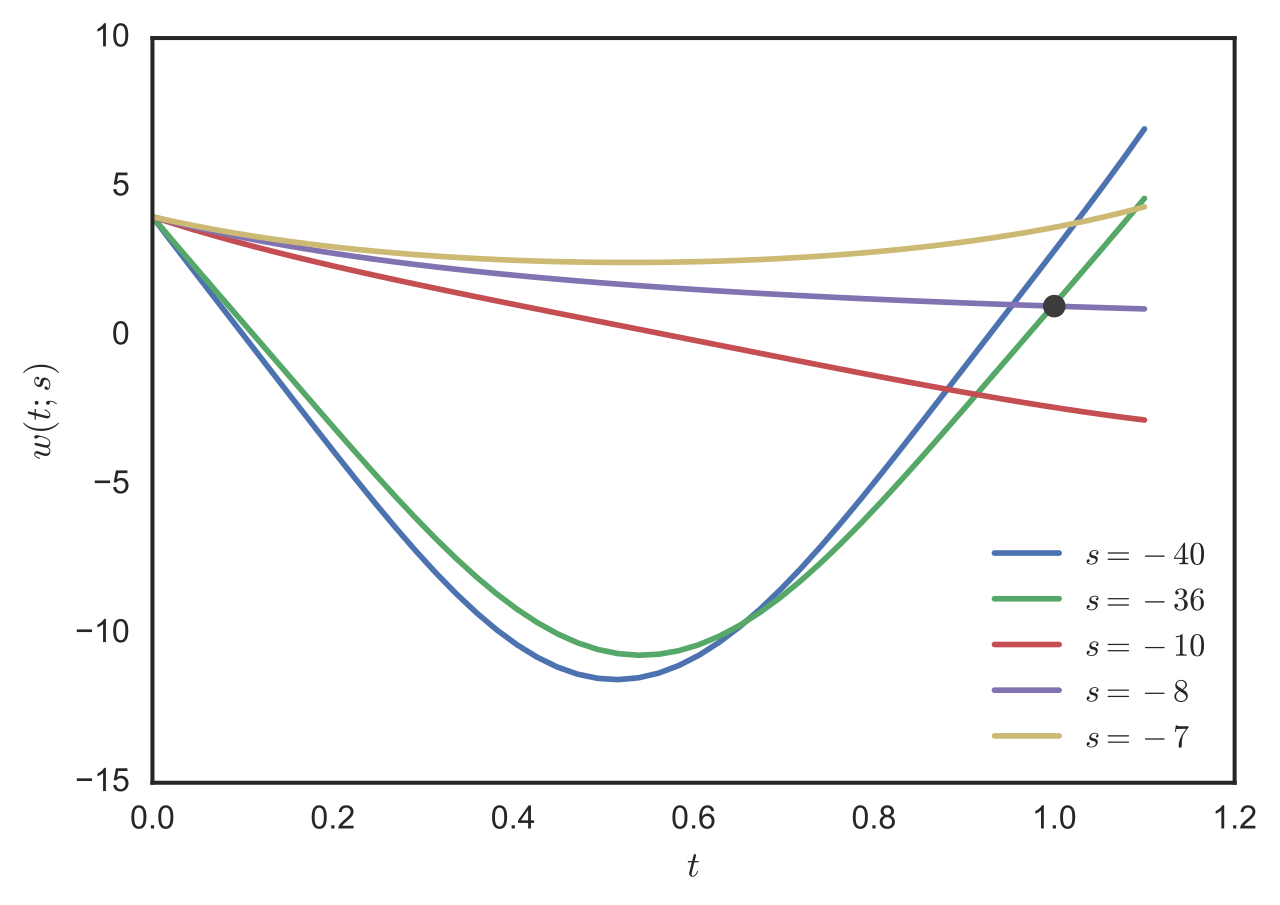
\includegraphics[width = 0.8\linewidth]{Images/shooting_ode_bvp.png}
    \item * Refer to SOLVING BVPs WITH THE ode45 INTEGRATOR AND SHOOTING* slides

\end{itemize}

End of the ODE section! \newline

\textbf{Monday}


\newpage
\def \secname {Basic Finite Difference Techniques for Time Dependent PDEs}

\section[\secname]{\hyperlink{toc}{\secname}}


We can divide time-dependent PDEs into two broad classes:
\begin{enumerate}
    \item \textbf{Initial-value Problems (Cauchy Problems)} spatial domain has no boundaries (either infinite or "closed" -- e.g. "periodic boundary conditions"
    \item \textbf{Initial-Boundary-Value Problems}, spatial domain \textit{finite}, need to specify boundary conditions
\end{enumerate}

\textbf{Note}: Even if \textit{physical} problem is really of Type 1, finite computational resources $\rightarrow$ finite spatial domain $\rightarrow$ approximate as Type 2; will hereafter loosely refer to either type as an IVP. \newline

\textit{Working Definition:} \textbf{Initial Value Problem}
\begin{itemize}
    \item State of physical system arbitrarily (usually) specified at some initial time $t=t_0$.
    \item Solution exists for $t \ge t_0$; uniquely determined by equations of motion (EOM) and boundary conditions (BCs).
\end{itemize}

\textit{Issues in Finite Difference (FD) Approximation of IVPs}

\begin{itemize}
    \item Discretization (Derivation of FDA's)
    \item Solution of algebraic systems resulting from discretization
    \item Consistency
    \item Accuracy
    \item Stability
    \item Convergence
    \item Dispersion/ Dissapation
    \item Treatment of Nonlinearities
    \item Computational Cost: Expect O(N) work, where N is the total number of spacetime grid points used
\end{itemize}

\subsection{Type of IVP (By example, 1 space fim and 1 time)}

\begin{itemize}
    \item Suppress boundary conditions for time being 
\end{itemize}

\subsubsection{Wave and Wave-like ("hyperbolic equations"): The 1-d wave equation}

\begin{equation}
     u_{tt} = c^2 u_{xx} \qquad u = u(t,x) \quad c \epsilon \mathcal{R}
\end{equation}

with initial conditions:
\[ u(x,0) = u_0(x)\]

\[ u_t(x,0) = v_0(x)\]

\subsubsection{Diffusion ("Parabolic"): The 1-d diffusion equation}

\begin{equation}
    u_t = \sigma u_{xx} \qquad \sigma \epsilon \mathcal{R}, \quad \sigma > 0
\end{equation}

with initial conditions:

\[ u(x,0) = u_o(x) \]

\subsubsection{Schrodinger: The 1-d Schrodinger equation}

\begin{equation}
    i \psi_t = - \frac{\hbar^2}{2m} \psi_{xx} + V(t,x) \psi \qquad \psi(t,x) \epsilon \mathcal{C}
\end{equation}

\[ \psi(x,0) = \psi_0(x)\]

\begin{itemize}
    \item Although $\psi(t,x)$ is complex in this case, can rewrite equation above as a system of 2 coupled scalar real-valued equations
\end{itemize}

\subsection{Basic Concepts: Definitions (mostly review)}

\subsubsection{Differential equation (ignoring BC's)}

forcing function, possible 0
\[ L_{LL} = f \]
where L term is a differential operator

\subsubsection{Difference equation (assume characterized by single discretization scale)}

F.D. operator here 
\[ L^hu^h = f^h\]

\subsubsection{Residual}

\begin{itemize}
    \item write FDA in canonical form
    \[ L^h u^h - h^h = 0\]

    \item $\Tilde{u} \Rightarrow$ be some approximation of $u^h$, then residual
    \[r^h \equiv L^h \Tilde{u}^h - h^h \qquad \Tilde{u}^h \rightarrow u^h; \quad r^h \rightarrow 0\]
\end{itemize}


\subsubsection{Truncation error (don't confuse with solution error)}

\begin{itemize}
    \item Truncation error $\tau^h$ of FDA is defined by 

    \[ \tau \equiv L^h u - f^h\]

    where u is the continuum solution

    \item Note: u satisfies the continuum D.E.

    \item  Form of T.E. can always be computed (Taylor Series) from the FDA and the D.E.
\end{itemize}

\subsubsection{Convergence}
\begin{itemize}
    \item Assume FDA characterized by single scale h, then $u^k$ converegs iff

    \[ u^h \rightarrow u \quad as \quad h\rightarrow0\]
\end{itemize}

\subsubsection{Consistency}

\begin{itemize}
    \item With same assumption, say FDA is consistent iff

    \[ \tau^h \rightarrow 0 \quad as \quad h\rightarrow 0\]

    \item Consistency is a necessary condition for convergence (not sufficient though) 
\end{itemize}

\subsubsection{Accuracy}

\begin{itemize}
    \item Assuming that the FDA is characterized by a single discretization scale, h, we say that the FDA is p-th order
    accurate or simply p-th order if

    \[ \text{lim}_{h\rightarrow0} \tau^h = O(h^p)\]
\end{itemize}

\subsubsection{Solution Error}

\begin{itemize}
    \item Solution error associated with FDA is

    \[ e^h \equiv u - u^h\]
    
\end{itemize}

\subsection{Sample Discretizations (FDAs): 1-d Differential Equation}

\begin{equation}
     u_{t} = \sigma u_{xx} \qquad (c=1) \qquad 0 \le x \le 1 ; \quad t\ge0
\end{equation}

\begin{itemize}
    \item Step 1: Discretize Domain (uniform grid) around points of form ($x_j, t^n)$ as shown in the figure below
\end{itemize}

\begin{figure}
    \centering
    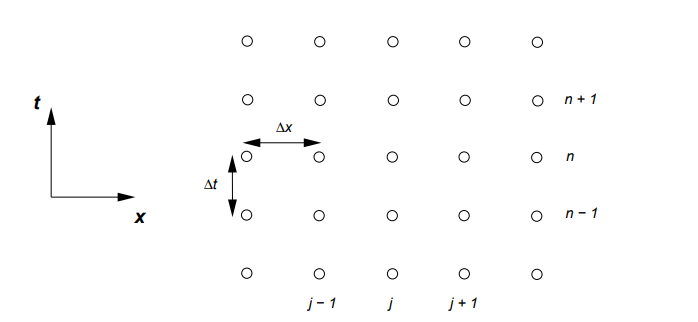
\includegraphics[width = 0.8 \linewidth]{Images/1dPDEwaveFDA_grid.png}
    \caption{Portion of uniform finite-difference mesh (grid) for 1-d time-dependent problem. Note that the spacings in both the spatial and temporal directions are constant}
    \label{fig:enter-label}
\end{figure}

\begin{align}
t^n &\equiv n \Delta t, & n &= 0, 1, 2, \ldots \\
x_j &\equiv (j-1)\Delta x, & j &= 1, 2, \ldots J \\
u_j^n &\equiv u((n-1)\Delta t, (j-1)\Delta x) \\
\Delta x &= (J-1)^{-1} \\
\Delta t &= \lambda \Delta x, & \lambda &\equiv \text{Courant number}
\end{align}

\begin{itemize}
    \item Step 2: Write down FDA for DE (see Figure \ref{fig:FDA_constr})
\end{itemize}

\begin{figure}
    \centering
    
\includegraphics[width = \linewidth]{Images/stencil_PDE_FDA.png}
    \caption{Stencil (molecule/star) for “standard” $O(h^2)$) approximation of (15).}
    \label{fig:FDA_constr}
\end{figure}


\textit{Discretized interior equation}:

\begin{align}
    \frac{u_j^{n+1}-u_j^n}{\Delta t} &= (u_{tt})_j^n + \frac{1}{2} \Delta t (u_{tt})_j^n + O (\Delta t^2) \\
    &= (u_{tt})_j^n + O (\Delta t)
\end{align}

\begin{align}
    \frac{u_{j+1}^n - 2 u_j^n + u_{j-1}^n}{\Delta x^2} &= (u_{xx})^n_j + \frac{1}{12} \Delta x^2 (u_{xxxx})_j^n + O(\Delta x^4)\\
    &= (u_{xx})_j^n + O(\Delta x^2)
\end{align}

FDA

\begin{equation}
    \frac{u_j^{n+1}-u_j^n}{\Delta t} = \sigma \frac{u_{j+1}^n - 2 u_j^n + u_{j-1}^n}{\Delta x^2}
\end{equation}

Where we can view the $u_j^{n+1}$ term as the equation for the unknown.

\begin{itemize}
    \item If we know $u_j^n$ for all j, then can compute $u_j^{n+1}$ for all j (given B.C.'s)
    \item Initialize scheme using

    \[ u_j^1 = u_0(x_j)\]

    where u is the given function

    \item Easy to solve explicitly for $u_j^{n+1} \Rightarrow$ Scheme is called explicit
\end{itemize}

*** Exam Hint Good question *** : 
\begin{itemize}
    \item Be able to discretize all continuum equations that that we use in class (for FDA)
    \item Be able to find the truncation error of these steps
\end{itemize}

Truncation Error
\begin{itemize}
    \item Interior equation

    \[ u_t = \sigma u_{xx} = (\partial_t - \sigma \partial_{xx})u = 0\]

    \item FDA
    \[ \p_t^h -\sigma \p_{xx}^h )u^h = 0 \]

    Where the partial terms in front of the u expression are the L operator and $L^u$ operator as discussed in the truncation section earlier.

    \item Truncation Error

\end{itemize}

\begin{align*}
    \tau ^h &\equiv L^h u \\
    &= (\partial_t^h - \sigma \partial^h_{xx}) u
\end{align*} 

\[ \tau ^h = (\partial_t^h - \sigma \partial^h_{xx}) u = (\partial_t - \sigma \partial_{xx}) u + \ldots \]

where the term in from of u equals to 0 $\Rightarrow$ consistency

\[ \tau^h = \frac{1}{2} \Delta t(u_{tt})^n_j - \frac{1}{12} \sigma \Delta x^2 (u_{xxxx})^n_j + O(\Delta t^2) + O(\Delta x^4)\]

above: Leading order truncation terms

\[ \tau^h= O(\Delta t) + O (\delta x^2) = O(\Delta t, \Delta x^2) \]

above: "First order in time; second order in space"

**"" Guranteed to be on final exam "" ** -Matt \newline

Discretize Boundary Conditions (Homogeneous Dirichlet):

\[ u_1^{n+1} = u_J^{n+1} = 0\]

Discretize Initial Conditions:

\[ u_j^1 = u_0(x_j)\]

Iterative solution procedure

set $u_j^1 \rightarrow u_j^2 \rightarrow u_j^3 \rightarrow \ldots$

Need solution not to blow up (will almost certainly be physical)

\subsection{Stability Analysis}

\begin{itemize}
    \item Heuristic notion of stability: size of numerical solution does not change "too much" as a function of time:

    \begin{equation}
        ||u(t,x)|| \sim  ||u(x,0)||
    \end{equation}

    Where $||\cdot||$ is some suitable norm, such that the $L_2$ norm

    \begin{equation}
        N(t) = ||u(t,x)|| \equiv \left( \int_0^1 u(t,x)^2 dx\right)^{1/2}
    \end{equation}

    \item Write time-dependent FDA in form 

    \[ \mathbf{u}^{n+1} = \mathbf{G}[\mathbf{u}^n],\]

    where $\mathbf{G}$ is some update operator (Matrix), and $\mathbf{u}$ is a column vector.

    \item Can always write FDA in this form by introducing auxiliary variables analogous to what we did for ODEs

    \item Solution at time step n can be written as

    \[ \mathbf{u}^n = \mathbf{G}^{(n-1)} \mathbf{u}^0\]

    \item Now, assume that G matrix has complete set of orthonormal eigenvalues:

    \[ \mathbf{e}_k, \quad k=1,2,\ldots J\]

    and associated eigenvalues 

    \[ \mu_k, \quad k = 1,2,\ldots, J\]

    so that 

    \[ \mathbf{G} \mathbf{e}_k = \mu_k \mathbf{e}_k \qquad k=1,2,\ldots, J\]

    \item Can now decompose initial data (spectral decomposition)

    \[ \mathbf{u}^0 = \sum_{k=1}^J c_k^0 \mathbf{e}_k\]
    \item then 

    \begin{align}
    \mathbf{u}^n &= \mathbf{G}^{n-1} \left(\sum_{k=1}^J c_k^0 \mathbf{e}_k \right) \\
    &= \sum_{k=1}^J c_k^0 (\mu_k)^{n+1} \mathbf{e}_k
    \end{align}

    Where we need the mu term to stay bounded. and the mu term could be complex.
    
    \item Clearly, if the scheme is to be stable, we must have

    \[ |\mu _k| \le 1 \qquad k=1,2, \ldots J\]
\end{itemize}

\begin{figure}
    \centering
    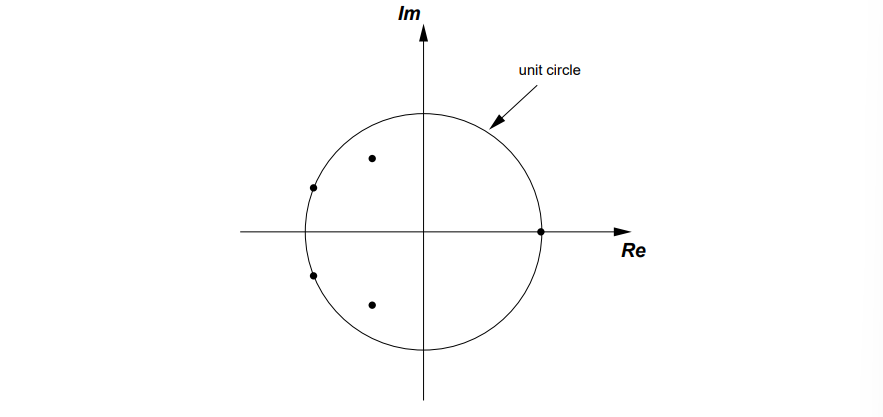
\includegraphics[width = \linewidth]{Images/complex_plane_eigenvalues.png}
    \caption{Schematic illustration of location in complex plane of eigenvalues of update matrix G. In this case, all eigenvalues (dots) lie on or within the unit circle, indicating that the corresponding finite difference scheme is stable.}
    \label{fig:enter-label}
\end{figure}

\subsection{Von-Neumann (Fourier) Stability Analysis}

\begin{itemize}

    \item Von-Neumann stability analysis is based on the ideas sketched in the figure, but additionally assumes
    \begin{itemize}
        \item that the difference equation is linear with constant coefficients,
        \item that the boundary conditions are periodic.
    \end{itemize}

    \item Can use Fourier Analysis: which has the same benefits in the discrete domain -- difference operators in real-space variable x $\rightarrow$ algebraic operations in Fourier-space variable k -- as it does in the continuum 
    
    \item Schematically, instead of 

    \[ \mathbf{u}^{n+1}(x) = \mathbf{G}[\mathbf{u}^n(x)],\]

    \item we consider the Fourier-domain equivalent

    \[ \tilde{\mathbf{u}}^{n+1}(k) = \tilde{\mathbf{G}}[\tilde{\mathbf{u}}^n(x)],\]

    \item where k is the wave number (Fourier-space variable). and the tilde denotes the Fourier transformed version of the different terms.

    \item Define Fourier-transform grid function via

    \begin{equation}
    \tilde{\mathbf{u}}^{n}(k) = \frac{1}{\sqrt{2 \pi}} \int_{\infty}^{\infty} e^{-ikx} \mathbf{u}^n(x) dx
    \end{equation}

    \item For a general difference scheme, we will find that

    \[ \tilde{\mathbf{u}}^{n+1}(k) = \tilde{\mathbf{G}}(\xi)\tilde{\mathbf{u}}^n(k)],\]

    \[ \xi = kh = k \Delta x\]

    Will need to show that $\tilde{\mathbf{G}}(\xi)$'s eigenvalues lie within or on the unit circle for all conceivable $\xi$.

    \item if $\tilde{\mathbf{G}}(\xi)$ is a scalar, then its modulus must be $\le 1$

    \[\tilde{\mathbf{G}}(\xi) \equiv \text{Amplification Matrix / Factor}\]

    \item What is appropriate range for $\xi = kh = k \Delta x$?

    \begin{itemize}
        \item Shortest wavelength representable on uniform mesh with spacing h is $\lambda=2h$ (Nyquist limit), corresponding to a maximum wave number $k = (2\pi )/\lambda = \pm \pi /h$.

        \item Therefore appropriate range is 

        \[ -\pi \le \xi \le \pi, \]
    \end{itemize}
    
    \item Start with VN stability analysis for diffusion equation from last day

    \item Introduce undivided difference operator $D^2$

    \[ D^2 u(x) = u(x+h) - 2u(x) + u(x-h)\]

    \item Supress spatial grid index, differential equation is 

    \[ u^{n+1} = u^n + \alpha D^2 u^n\]
    \[ \alpha = \sigma \frac{\Delta t}{h^2} = \sigma \frac{\Delta t}{\Delta x^2}\]

    \item What's action of $D^2$ in fourier space?

    \item Use inverse F.T.

    \[ u(x) = \frac{1}{\sqrt{2 \pi}} \int_{-\infty}^{\infty} e^{ikx}\tilde{k}dk\]
    so 

    \begin{align}
        D^2 u(x) = u(x + h) - 2u(x) + u(x - h) &= \int_{-\infty}^{\infty} (e^{ikh} - 2 + e^{-ikh})e^{ikx}\tilde{u}(k)dk\\
        &= \int_{-\infty}^{\infty} (e^{i \xi} - 2 + e^{-i\xi}) e^{ikx}\tilde{u}(k)dk
    \end{align}

    \item We can replace the term in brackets with $-4\sin^2(\xi/2)$:

    \[ D^2 u(x) = u(x + h) - 2u(x) + u(x - h) = \int_{-\infty}^{\infty} \left(-4\sin^2(\xi/2)\right)e^{ikx}\tilde{u}(k)dk\]

    \item Missed some points

    \item Amplificaiton Factor in Fourier space:

    \begin{equation}
        \tilde{\mathbf{G}} = 1-4 \alpha \sin^2(\xi/2)
    \end{equation}

    \item Thus, for stability must have

    \[ 4 \alpha \sin^2 (5/2) \le 2 \quad \rightarrow \quad \alpha \le \frac{1}{2}\]

    \begin{equation}
        \alpha = \sigma \frac{\Delta t}{\Delta x^2} \le \frac{1}{2}
    \end{equation}

    \item But of bad news: as $\Delta x \rightarrow 0 , \Delta t$ must $\rightarrow 0$ quadratically in $\Delta x$
    \item In following, will drop integrals, $\frac{1}{\sqrt{2\pi}}$, $e^{ikx}$ and simply write down amplification matrix when it is clear what it is
\end{itemize}

\subsection{Some other discretizations of the diffusion equation}

\subsubsection{Implicit First-Order}

\begin{itemize}
    \item One general way to improve stability of FDAs is to use implicit schemes
    \item Use same mesh, different stencil

    \item FDA

    \[ \frac{u_j^{n+1}-u_j^{n}}{\Delta t} = \sigma \frac{u_{j+1}^{n+1}-2u_j^{n+1}+u_{j-1}^{n+1}}{\Delta x^2}\]

    \item Perform T.S. expansions about $(x_j, t^{n+1})$ get T.E. (verify!)

    \[ \tau = - \frac{1}{2} \Delta t(u_{tt})^{n+1}_{j} + \frac{1}{12} \sigma \Delta x^2 (u_{xxxx})_j^{n+1} + O(\Delta t^2)+ O(\Delta x^2)\]

    \[ \tau = O(\Delta t, \Delta x^2)\]

    First order in time, second order in space

    \item Can't explicitly write down formula for $u_j^{n+1}$ due to coupling of unknowns at $t=t^{n+1}$

    \item Scheme is implicit 

    \item Have to solve (linear) system of equations for $u_j^{n+1}, \qquad j = 1,2,\ldots , J$

    \item Defer solution discussion until stability properties derived

    \item Write scheme as

    \[ u_j^{n+1} = u_j^n + \alpha D^2 u_j^{n+1}\]

    where we are using $\alpha, \quad D$ as previously mentioned

    \[ \Rightarrow (1-\alpha D^2) u^{n+1} - u^n\]

    \item Now apply F.T., get (verify!)

    \[ (1+4\alpha \sin^2 \frac{\xi}{2} \tilde{u}(k)^{n+1} = \tilde{u}(k)^n\]

    \item So, amplification factor is 

    \[ \tilde{G}(\xi) = \frac{1}{1+4\alpha \sin^2\frac{\xi}{2}}\]

    \[ \Rightarrow \tilde{G}(\xi) \le 1 \text{ For ALL } \alpha, \xi\]

    Such a scheme is said to be unconditionally stable (in the VN sense)

    \item VN stability necessary but not necessarily sufficient for "True" stability.

    \textbf{October 30th 2023}

    \item Set $\sigma = 1$ and rearrange earlier equation:
    \[ (-\Delta x^{-2}) u_{j+1}^{n+1} + (\Delta t^{-1} + 2 \Delta x^{-2})u_j^{n+1} +(-\Delta x^{-2})u_{j-1}^{n+1} = (\Delta t^{-1}) u_j^n , \qquad j=2,\ldots, J-1 \]

    \[ u_1^{n+1} = u_J^{n+1} = 0 \qquad \text{(Homogeneous, Dirichlet. B.C.;}\]

    \item In matrix form

    \[ \mathbf{A} \mathbf{u}^{n+1} = \mathbf{b}\]

    What is the structure of matrix A? (non-zero)

    \begin{itemize}
        \item Tri-diagonal system. i.e. three diagonals but everything else is 0.
    \end{itemize}

    \item Special case of \textbf{sparse} matrix, defined as a matrix with a majority of 0 elements (roughly 50 percent or more)

    \item Here, for large J, vast majority of elements will be 0.

    \item Can optimize solution of linear system W.R.T. the sparsity structure

    \item For tridiagonal systems can compute solution in $O(J)$ time vs general $O(J^3)$, BUT have to take advantage of sparsity structure

    \item Recommended approach in MATLAB:

    \begin{verbatim}
        spdiags  % (sparse diagonals)
    \end{verbatim}
    \item Illustrate using example which solves above system ($nx=J$)

    \item Define diagonals of sparse matrix $\mathbf{A}$ as columns of auxiliary matrix $\mathbf{B}$, pass $\mathbf{B}$ along with diagonal numbers to spdiags

    \begin{verbatim}
        % Initialize storage for sparse matrix and RHS

        dl = zeros(nx, 1);
        d = zeros(nx,1);
        du = zeros(nx,1);
        f = zeros(nx,1);

        % Set up tridiagonal system

        dl = -1.0/dx^2 * ones(nx,1);
        d = (1.0/dt * 2.0/dx^2) * ones(nx,1);
        du = dl;

        % Fix up boundary cases

        % Left B.C.
        d(1) = 1.0;
        du(2) = 0.0;

        % Right B.C.
        dl(nx-1) = 0.0;
        d(nx) = 1.0;

        % Define sparse matrix
        % B is [dl d du]
        % -1:1 is which diagonals 
        % nx, nx is dimensions

        A = spdiags([dl d du], -1:1, nx, nx)

        % Define RHS vector 

        f(2:nx-1) = u(n, 2:nx-1)/dt;
        f(1) = 0;
        f(nx) = 0;
    \end{verbatim}

    \item Can then use $\mathbf{A}$ in linear solve via left division

    \begin{verbatim}
        u(n+1,:) = A\f;

        % \ operator knows about sparse matrices; solve is optimized, very fast!
    \end{verbatim}

    \item Can see full matrix (with all 0's included using the full command:

    \begin{verbatim}
        full(A)
    \end{verbatim}

    \item Diagonal in position M from main diagonal has length nx-m
    \item Thus, any column of $\mathbf{B}$ other than the main diagonal will have positions/values that are not used

    \item Diagonal above (super diagonal): At beginning
    \item Diagonal below (sub diagonal): At end

    \item Once more, note how B.C's are implemented

    \[(1)u_1^{n+1} + (0) u_2^{n+1} = 0\]

    \[ (0) u_{J-1}^{n+1} + (1) u_{J}^{n+1} = 0\]
\end{itemize}

\subsubsection{Crank-Nicholson Scheme}

\begin{figure}
    \centering
    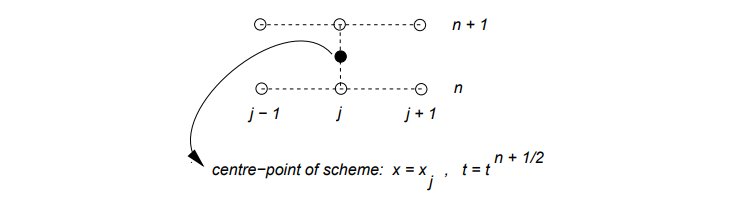
\includegraphics[width = \linewidth]{Images/crank_nicholson_scheme.png}
    \caption{: Stencil (molecule/star) for $O(h^2)$ Crank-Nicholson approximation of (19)}
    \label{fig:crank-nicholson}
\end{figure}

\[ u_t = \sigma u_{xx}\]

Using rectangle stencil with center fictitious point at n+1/2 and j. And that is where you do the taylor series about.

\textbf{FDA}

\begin{equation}
    \frac{u_j^{n+1}-u_j^n}{\Delta t} = \frac{1}{2} \sigma \left[ \frac{u_{j+1}^{n+1} - 2u_j^{n+1} + u_{j-1}^{n+1}}{\Delta x^2} + \frac{u_{j+1}^n-2u_j^n+u_{j-1}^n}{\Delta x^2} \right]
\end{equation}

\textbf{November 1st 2023}

Truncation error takes quite a bit of work; here is the result:

\[ \tau = \frac{1}{24} \Delta t^2 (u_{ttt})_j^{n+\frac{1}{2}} - \frac{1}{8} \sigma \Delta t^2 (u_{ttxx})_j^{n+\frac{1}{2}} - \frac{1}{12} \sigma \Delta x^2 (u_{xxxx})_j^{n+\frac{1}{2}}+O(\Delta t^4) + O(\Delta x^4) + O(\Delta t^2 \Delta x^2)\]

\[ \tau = O(\Delta t^2, \Delta x^2) \Rightarrow \text{ Improved temporal accuracies relative to first two schemes}\]

\begin{itemize}
    \item "Wouldnt ask to derive a truncation error for a scheme like this on the exam but he WOULD ask for us to derive truncation error for previous two schemes"
    \item Make sure you can derive tau for simpler (first order) schemes, ** Exam Hint **
\end{itemize}

Stability
\begin{itemize}
    \item Write scheme
    \[(1- \frac{\alpha}{2} D^2 ) u_j^{n+1} = (1+\frac{\alpha }{2} D^2) u_j^n\]

    $\alpha, \quad D^2$ as previously used
    \item Apply Fourier Transform (get $\rightarrow$ verify)
    
    \[(1+2\alpha \sin^2 \xi/2 ) \tilde{u}(k)^{n+1} = (1-2\alpha \sin^2\xi/2 ) \tilde{u}(k)^n\]
    
    \item Amplification factor is
    \[ \tilde{G}(\xi) = \frac{1-2\alpha \sin^2 \xi/2}{1+2\alpha \sin^2 \xi/2} \]
    \item This is of the form
    \[ \tilde{G}(\xi) = \frac{1-x}{1+x} \qquad x \ge 0 \]

    \[ \tilde{G}(\xi) \le 1 \text{ for all } \xi, \alpha \]

    Scheme is also \textbf{unconditionally} stable

    \item Solution with Crank method yields same structure as the t grid 

    $\Rightarrow$ tridiagonal system

    \item Solve using spdiags as we did for implicit scheme (tutorial next week)
\end{itemize}

\subsubsection{Exact Solution for Testing}

\begin{itemize}
    \item Recall 

    \[ u_t = \sigma u_{xx}\]
    on
    \[ 0 \le x \le 1 \qquad t\ge 0\]

    \[ u(x,0) = u_0(x)\]
    \[u(0,t) = u(1,t) = 0\]

    \item Exact solution

    \[ u(x,t) = e^{-\sigma \omega ^2 t} \sin(\omega t) \]

    where $\omega = n \pi , \qquad n=1,2, \ldots$

    \[ u_t = u_{xx} = -\sigma \omega^2 u(t,x)\]
\end{itemize}


\subsection{The 1-D Schr\"{o}dinger Equation}

\begin{equation}
    i \psi_t = - \frac{\hbar^2}{2m} \psi_{xx} + V(t,x) \psi
\end{equation}

\[ 0 \le x \le 1\]

\[ \psi(t,x) \in \mathbb{C}\]

\[ \text{V(t,x) is given potential} \]

\begin{itemize}
    \item Non-dimensionalize, solve on unit interval with homogeneous Dirichlet B.C.'s 

    \[ i \psi_t = - \psi_{xx} + V \psi \]

    

    \[ \psi(0,x) = \psi_0(x)\]

    \[ \psi(t,0) = \psi(t,1) = 0 \Rightarrow \text{Physical interpretation?}\]

    Infinite potential walls at x=0, 1; no penetration of wave function

    \item Exact solution for testing (V=0)
    \[ \psi(t,x) = e^{i\omega ^2 t } \sin(\omega x)\]

    where $\quad \omega = n \pi , \quad n=1,2,\ldots$

    \textbf{FDA:}

    Use crank-nicholson grid

    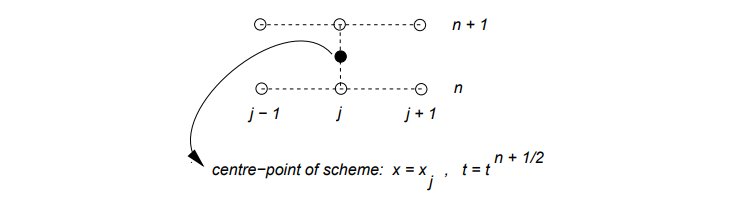
\includegraphics[width =  \linewidth]{Images/crank_nicholson_scheme.png}
    

    \[ \psi_j^{n+\frac{1}{2}} = \frac{1}{2} ( \psi^{n+1}_j + \psi_j^n)\]

    with error of $O(\Delta t^2)$


    \begin{equation}
        i \frac{\psi^{n+1}_j-\psi^n_j}{\Delta t} = -\frac{1}{2}\left( \frac{\psi^{n+1}_{j+1} - 2 \psi_j^{n+1} + \psi _ {j-1}^{n+1}}{\Delta x^2} + \frac{\psi_{j+1}^n-2\psi_j^n + \psi_{j-1}^n}{\Delta x^2}\right) + \frac{1}{2} V_j^{n+\frac{1}{2}} (\psi_j^{n+1}+\psi_j^n) 
    \end{equation}

    \[ \psi^{n+1}_j = \psi^{n+1}_J = 0\]

    \item Truncation error 

    \[ \tau = O(\Delta t^2, \Delta x^2)\]

    Second order in space and time

    \item Stability analysis

    \item \textbf{Theorem}: In stability analysis, can neglect terms that do not include spatial derivatives!

    \item EXAM HINT FOR 830AM final: "undifferentiated terms you don't need to worry about... etc for stability analysis"

    \item Write scheme, without $V \psi$ term, as 

    \[ (i + \frac{1}{2} \alpha D^2) \psi^{n+1} = (i-\frac{1}{2} \alpha D^2) \psi^n\]

    $D^2 $ as before \newline

    $\alpha = \frac{\Delta t}{\Delta x^2}$

    \item Under F.T.

    \[ (i- 2 \alpha \sin^2 \xi/2 ) \tilde{\psi}(k)^{n+1} = (i+2\alpha \sin^2 \xi/2) \tilde{\psi}(k)^n\]
    

    \item Read off amplification factor 

    \[ \tilde{G}(\xi) = \frac{i+2\alpha \sin^2 \xi/2 }{i-2\alpha \sin^2 \xi/2}\]

    Which is of the form

    \[ \frac{1+a}{1-a} \qquad a \text{ REAL}\]
    \[ \left| \frac{i+a}{i-a} \right| = \frac{|i+a|}{|i-a|} = \frac{1+a^2}{1+a^2} = 1\]

    Thus,

    \[ |\tilde{G}(\xi)| = 1 \quad \text{ for all } \xi, \alpha\]

    The scheme is unconditionally stable

    This reflects fact that probability is conserved in the continuum

    "we will see this in play with final project"

    Solution of equations

    \item Rewrite equation as tridiagonal system

    \[ C^+_j \psi_{j+1}^{n+1} + C_j^0 \psi _j^{n+1} + c_j^- \psi_{j-1}^{n+1} = f_j\]

    where only second term of c has actual j dependence from the V psi term

    \item Set up matrix using spdiags, solve using left division (project )
\end{itemize}

\subsection{Wave-equation}

\subsubsection{1-D Wave equation with fixed (dirichlet) B.C.'s}

\[ u_{tt} = u_{xx} \qquad (c=1) \qquad 0 \le x \le 1 \quad t \ge 0\]

\[ u(0,x) = u_0(x)\]

\[ u_t(0,x) = u_0(x)\]

\[ u(t,0) = u(t,1) = 0\]

\begin{itemize}
    \item Step 1: Discretize domain (use same mesh)

    \item Make FDA Characterized by single scale, h

    \[ \Delta t = \lambda \Delta x = \lambda h\]

    \[ h = \Delta x\]

    \[ \lambda = \frac{\Delta t}{\Delta x}\]

    \[ \lambda \equiv \text{"Courant Number"}\]

    \item Whenever we vary $\Delta x$, automatically vary $\Delta t$ ($\lambda$ held constant)

    \item Step 2: Write down FDA:
    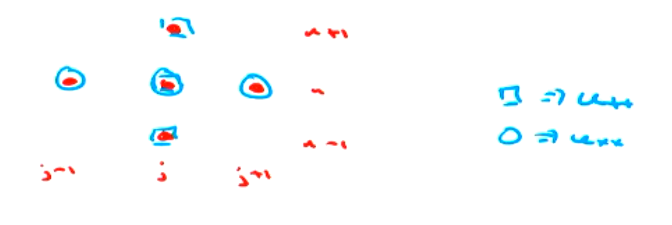
\includegraphics[width = \linewidth]{Images/wave_fda.png}


    MAKE SURE YOU CAN DERIVE THIS FOR EXAM HINT  - if you know the left hand side, also know how to get the expansion on the right hand side***

    
    \[ (\Delta t)^{-2} ( u_j^{n+1}-2u_j^n+u_j^{n-1}) = (u_{tt})_j^n + \frac{1}{12} \Delta t^2 (u_{tttt})_j^n + O(\Delta t^4)\]

    \[ = (u_{tt})_j^n+O(\Delta t^2)\]


    hint: Same expansion (can use similarity argument on exam and not repeat full derivation): 

    
    \[ (\Delta x)^{-2} ( u_{j+1}^{n}-2u_j^n+u_{j-1}^{n}) = (u_{xx})_j^n + \frac{1}{12} \Delta x^2 (u_{xxxx})_j^n + O(\Delta x^4)\]

    \[ = (u_{xx})_j^n+O(\Delta x^2)\]


    \item FDA

    \[ \frac{u_j^{n+1}-2u_j^n+u_j^{n-1}}{\Delta t^2} = \frac{u_{j+1}^n - 2 u_j^n + u_{j-1}^n}{\Delta x^2} \qquad j=2,3,\ldots, J-1\]

    \item Called a ``three level scheme'' since it couples unknowns on 3 time levels 

    \item Truncation error ($\tau = \tau^h = L^h u $; $L^hu^h = 0$)

    First write FDA in form

    \[ \tau = \frac{1}{12} \Delta t^2 (u_{tttt})_j^n - \frac{1}{12}\Delta x^2 (u_{xxxx})_j^n + O(\Delta t^4) + O(\Delta x^4)\]

    \[ = O(\Delta x^2, \Delta t^2) = O(h^2)\]

    Second order in space and time

    \item Discrete B.C.'s 

    \[ u_1^{n+1} = u^{n+1}_J = 0\]

    Missed info 

    \item Discrete I.C.'s

    \begin{itemize}
        \item Need to give two ``time levels" of data (effectively $u(0,x), u_t(0,x)$

        \[ u_j^1 \quad , \quad j=1,2, \ldots , J\]

        \[ u_j^2 \quad , \quad j=1,2, \ldots , J\]
    \end{itemize}

    \item Can solve FDA equation above for $u_j^{n+1}$ explicitly

    \[ u_j^{n+1} = 2u_j^n -u_j^{n-1} + \lambda^2 ( u_{j+1}^n - 2u_j^n + u_{j-1}^n)\]

    \item Initialization revisited 

    \item First time level: $u_0(x)$

    \[ u_j^1 = u_0(x_j)\]

    Second time level: need to determine $u_j^2$ up to and including $O(\Delta t^2)$ terms

    \begin{align}
        u_j^2 &= u_j^1 + \Delta t (u_t)_j^1 + \frac{1}{2} \Delta t^2 (u_{tt})_j^1 + O(\Delta t^3) \\
        &= u_j^1 + \Delta t (u_t)_j^1 + \frac{1}{2} \Delta t^2 (u_{xx})_j^1 + O(\Delta t^3)\\
        &= u_0(x_j) + \Delta t v_0(x_j) + \frac{1}{2} \Delta t^2 u_0''(x_j)
    \end{align}
\end{itemize}

Stability Analysis 
(more involved due to 3 time levels)

\begin{itemize}
    \item Rewrite FDA in ``first order" form by introducing auxiliary variables

    \[ v_j^n = u_j^{n-1} \Rightarrow v_j^{n+1}=u_j^n\]

    \[ \Rightarrow u_j^{n+1} = 2 u_j^n - v_j^n + \lambda^2(u_{j+1}^n - 2u_j^n + u_{j-1}^n)\]

    \[ v_j^{n+1} = u_j^n\]

    \item In matrix form

    \[\begin{bmatrix}
        u \\
        v
    \end{bmatrix}^{n+1} = \begin{bmatrix}
        2+\lambda^2D^2-1 & -1 \\
        1 & 0
    \end{bmatrix}
    \begin{bmatrix}
        {u} \\
        {v}
    \end{bmatrix}^n \]

    Where the D terms is same as $D^2$ previously 
    
    \item Under Fourier Transormation, becomes

    \[\begin{bmatrix}
        \tilde{u} \\
        \tilde{v}
    \end{bmatrix}^{n+1} = \begin{bmatrix}
        2-4\lambda^2 \sin^2 \xi/2 & -1 \\
        1 & 0
    \end{bmatrix}
    \begin{bmatrix}
        \tilde{u} \\
        \tilde{v}
    \end{bmatrix}^n\]

    where the matrix is $\tilde{G}(\xi)$

    \item Need to determine conditions so $\tilde{G}(I)$ has eigenvalues on or within unit circle

    \item Characteristic equation (whose roots are the e.v.'s)

    \[ \begin{vmatrix}
    2-4\lambda^2\sin^2\xi/20-\mu & -1 \\
    1 & \mu
        
    \end{vmatrix} = 0
    \]

    or

    \[ \mu^2 + (4 \lambda^2 \sin^2\xi/2 -2 ) \mu + 1 = 0\]
    Equation has roots at

    \[ \mu ( \xi) = (1-2\lambda^2 \sin^2 \xi/2 ) \pm ((1-2\lambda^2 \sin^2 \xi/2)^2 -1)^{1/2}\]

    Need sufficient conditions for

    \[ |\mu(\xi)| \le 1\]
    Equivalently

    \[ |\mu(\xi)|^2 \le 1\]

    \[ \mu(\xi) = (1-Q) \pm ((1-Q)^2-1)^{1/2} \]

    \[ Q\equiv 2 \lambda^2 \sin^2 \xi/2\]

    \item 3 cases to consider

    \begin{enumerate}
        \item \[(1-Q)^2-1 = 0\]

        \item \[(1-Q^2)-1 < 0\]

        \item \[ (1-Q^2)-1 > 0\]
    \end{enumerate}

    Case 1: $Q=0$ or $Q=2$, In both cases $|\mu(\xi)|=1$

    Case 2: $((1-Q)^2-1)^{1/2}$ purely imaginary

    \[ \mu(\xi) = (1-Q)^2 + (1-(1-Q)^2) = 1\]

    Case 3: $(1-Q)^2 -1 > 0 \rightarrow (1-Q)^2 > 1 \rightarrow Q>2$

    \[ 1-Q - ((1-Q)^2-1) < -1\]

    Instability at
    \[ |\mu(\xi)| > 1\] 

    \item Necessary condition for von Neumann stability

    \[ (1-Q)^2 -1 \le 0 \rightarrow (1-Q)^2 \le 1 \rightarrow Q \le 2\]

    \item But $Q=2\lambda^2 \sin^2 \xi/2 \quad ; \quad 2 \lambda^2 \le 2 ; \quad \lambda^2 \le 1$

    For stability we need
    \[ \lambda \equiv \frac{\Delta t}{\Delta x} \le 1\]

    \item This condition is often called the CFL condition—after Courant, Friedrichs and Lewy who derived it in 1928 (the ratio $\lambda = \Delta x/ \Delta t$ is also frequently called the \textit{Courant number}). In practical terms, we must limit the time-discretization scale , $\Delta t$, to values no larger than the space-discretization scale, $\Delta x$. Furthermore, this type of instability has a “physical” interpretation, often summarized by the statement \textit{the numerical domain of dependence of an explicit difference scheme must contain the physical domain of dependence}.

    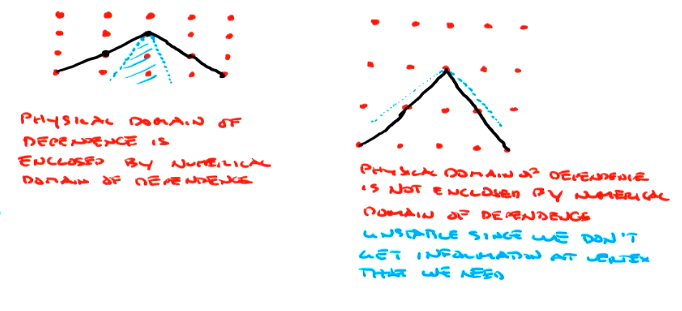
\includegraphics[width = 0.9 \linewidth]{Images/CFL_condition.png}

    \item EXAM HINT : make sure you can do a stability analysis like this!! Really good exam question

\end{itemize}

\textbf{November 6th 11:19am}

\subsection{Dispersion in FDAs}

\begin{itemize}
    \item Advection Equation

    \[ u_{t} = a u_x\]

    \item Exact solution

    \[u(t,x) = f(at+x)\]

    Propogates initial data profile to the left with speed a. No change in profile's shape $\Rightarrow$ non-dispersive. Every fourier component travels with the same speed c.

    \item Semi-discretization: only discretize in space

    \[ u_t = a D_x u = a \frac{u_{j+1}-u_{j-1}}{2\Delta x}\]
    Leave time continuous

    \item Look for normal mode solutions, of the form

    \[ u = e^{ik(x+G't)}\]

    $k \equiv $ to the wave number \newline
    $a' \equiv $ to the discrete phase speed associated with k

    \item Substitute in (a')

    \[ ika' u = \frac{a (2 i \sin(k \Delta ))}{2\Delta x} u \]

    \item Solve for a'

    \[ a' = a \frac{\sin(k \Delta x)}{k\Delta x} = a \frac{\sin\xi}{\xi}\]

    \[ \xi \equiv k \Delta x\]

    \item Low frequency limit $\xi \rightarrow 0$

    \[ a' = \lim_{\xi\rightarrow0} a \frac{\sin\xi}{\xi} = a \]

    Expected result

    \item High frequency limit, $\xi \rightarrow \pi$

    \[ a' = a \frac{\sin \pi}{\pi} = 0 \]

    Highest frequency components don't propagate at all

    \item Typically of low-order FDAs

    \item In practice may want to damp high-frequency components by adding explicit dissipation to the scheme

    \item High-frequency components often responsible for instabilities
\end{itemize}

End of discussion about PDEs in 1-D

\newpage
\def \secname {Solution of problems in two space dimensions}

\section[\secname]{\hyperlink{toc}{\secname}}




Time-dependent equation that we study, diffusion equation, will serve as a model for the solution of the Schroedinger Equation that we will solve in the Project 2.

\subsection{Diffusion Equation}

\begin{itemize}
    \item Model Equation

    \[ y(x,y,t)_t = \nabla ^2 u = u_{xx} + u_{yy}\]

    \[ u_t = u_{xx} + u_{yy} \qquad \sigma = 1\]

    where sigma is the diffusion constant.

    On 

    \[ 0 \le x \le 1, \quad 0 \le y \le 1; \quad t\ge 0\]

    Subject to 

    \[ u(x,y,0) = u_0(x,y)\]

    \[ u(0,y,t) = u(1,y,t) = u(x,0,t) = u(x,1,t) = 0\]

    \item Solve by FDA

    \item Step 1: Discretize Domain

    Spatial Mesh

    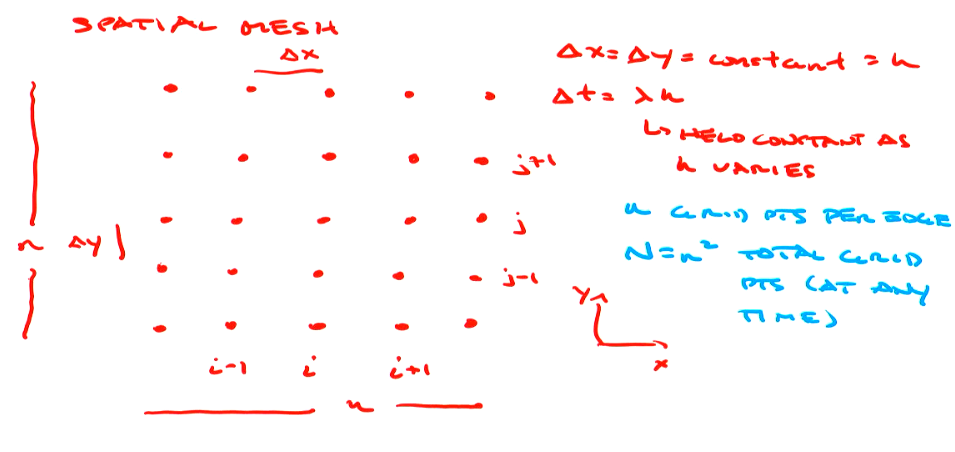
\includegraphics[width  = \linewidth]{Images/2D_spatialmesh_diffusion.png}

    \begin{equation}
        \begin{bmatrix}
            u_{1,1} \\
            \vdots \\
            u_{n,1} \\
            \vdots \\
            u_{1,n} \\
            \vdots \\
            u_{n,n}
        \end{bmatrix} = \mathbf{u}^n \qquad n^2 = N \text{ components}
    \end{equation}
    \item Grid Function notation

    \[ u_{i,j}^n = u(x_i, y_j, t^n)\]
\end{itemize}

\subsection{The Crank-Nicholson Scheme For 2D Diffusion Equation}

\begin{itemize}
    \item Assume retains 1-D properties: second-order accuracy, unconditional stability

    \item Introduce F.D. operators: $\p_{xx}^h$, and $\p_{yy}^h$

    \[ \p_{xx}^h u_{i,j}^n =  \frac{ u^n_{i+1,j} - 2u^n_{i,j}+u^n_{i-1,j}}{\Delta x^2}\]

    \[ \p_{yy}^h u_{i,j}^n = \frac{ u^n_{i+1,j} - 2u^n_{i,j}+u^n_{i-1,j}}{\Delta y^2}\]

    \item Then scheme is 

    \[ \frac{u_{i,j}^{n+1}-u_{i,j}^n}{\Delta t} = \frac{1}{2} ( \p_{xx}^h + \p_{yy}^h ) ( u_{i,j}^{n+1} + u_{i,j}^n)\]

    Centre point of scheme

    \[ (x_i, y_j, t^{n+\frac{1}{2}})\]

    \item Truncation error ($\Delta x = \Delta y$)

    \[ \tau = \frac{1}{24} \Delta t^2 (u_{ttt})_{i,j}^{n+\frac{1}{2}} - \frac{1}{8} \Delta t^2 ((u_{ttxx})_{i,j}^{n+\frac{1}{2}}+ (u_{ttxx})_{i,j}^{n+\frac{1}{2}}) - \frac{1}{12} \Delta x^2 ((u_{xxxx})_{i,j}^{n+\frac{1}{2}} + (u_{yyyy})^{n+\frac{1}{2}}_{i,j}) + O(h^4)\]

    \[ = O(\Delta t^2, \Delta x^2) = O(h^2)\]

    Second order in space and time

    \item Define 

    \[ L^h \equiv \p_{xx}^h + \p_{yy}^h\]

    The scheme can be written as 

    \[ (1- \frac{\Delta t}{2} L^h) u_{i,j}^{n+1} = (1+ \frac{\Delta t}{2} L ^h) u_{i,j}^n\]

    Represents linear system of equations for $u_{i,j}^{n+1}$

    \[ \mathbf{A} \mathbf{u}^{n+1} = \mathbf{b}\]

    Where the u vector is all unknown $u_{i,j}^{n+1}$ arranged row by row E.G.

    \item $\mathbf{A}$ will again be sparse; what is its sparsity structure?

    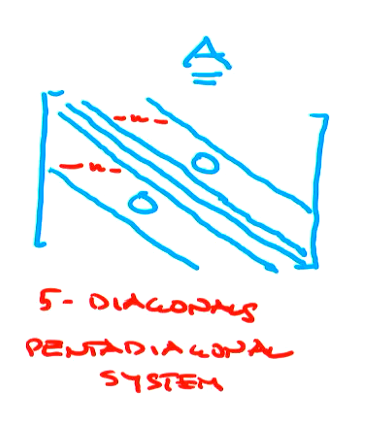
\includegraphics[width = 0.5\linewidth]{Images/pentadiagonal.png}

    Think coupling with nearest neighbour left and right $\pm 1$ and then also above and below $\pm n$ (unlikely to ask this on the final exam)
    
    \item What is cost of solving systems ? (Recall in 1-D we had tridiagonal system, cost was $O(n) = O(N) \Rightarrow$ Optimal); here $O(n^2) = O(N)$ is optimal

    \item Bandwidth, W, of matrix is total number of diagonals that span non-zeros portion

    \item For constant bandwidth NxN systems can be solved in $O(c_w N)$ time when $c_w$ is a constant that depends on $c_w$; $c_w$ is quadratic in $w$

    \textbf{November 8th 2023, 11am}

    \item $c_w \sim n^2$ so the order is still $O(N^2)$ 

    \item $\Rightarrow$ Direct solution of the linear system even taking into account sparsity structure is too expensive

    \item IDEA: operator on left is schematically 

    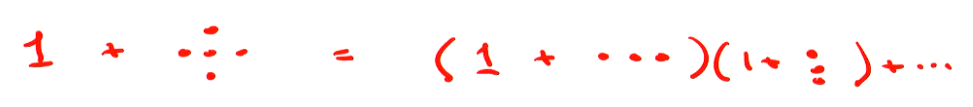
\includegraphics[width = 0.9 \linewidth]{Images/operator_schematic.png}

    
\end{itemize}

\subsection{Altenating direction implicit method for the diffusion equation}

**Hint for Project 2, try this before trying for Project 2** \newline

Factor operator on left into 1-D operators $\Rightarrow$ resulting linear systems are tridiagonal and can be solved efficiently.

\[ (1-\frac{\Delta t}{2} L^h) u_{i,j}^{n+1} = (1+ \frac{\Delta t}{2} L^h) u_{i,j}^{n}\]

\begin{itemize}
    \item Recall: $L^h = \p_{xx}^h + \p_{yy}^h$, so factor

    \[ (1-\frac{\Delta t}{2} \p_{xx}^h)(1-\frac{\Delta t}{2} \p_{yy}^h) u_{i,j}^{n+1} = (1+\frac{\Delta t}{2} \p_{xx}^h)(1+\frac{\Delta t}{2} \p_{yy}^h) u_{i,j}^{n} + \frac{\Delta t^2}{4} \p_{xx}^h \p_{yy}^h (u_{i,j}^{n+1}-u_{i,j}^n)\]

    where the last added term are the quadratic terms from factorization ($O(\Delta t^3)$

    \[ u_{i,j}^{n+1} = u_{i,j}^{n} + \Delta t(u_t)_{i,j}^2 + O(\Delta t^2)\]

    \[ u_{i,j}^{n+1} - u_{i,j}^{n} = O(\Delta t) \]

    So we have

    \[ (\qquad )(\qquad ) u_{i,j}^{n+1} = (\qquad)(\qquad)u_{i,j}^{n} + O(\Delta t^2)\]

    This defines the one-step update $\Rightarrow$ for $O(\Delta t^2)$ global error can neglect $O(\Delta t^2)$ term

    Gives one for of ADI scheme

    \begin{equation}
        (1-\frac{\Delta t}{2} \p_{xx}^h )(1-\frac{\Delta t}{2}\p_{yy}^h) u_{i,j}^{n+1} = (1+\frac{\Delta t}{2} \p_{xx}^h)(1+\frac{\Delta t}{2} \p_{yy}^h) u_{i,j}^{n}
    \end{equation}

    \item Solve in stages: introduce intermediate grid function $u_{i,j}^{n+\frac{1}{2}}$

    let;

    \begin{equation}
        (1-\frac{\Delta t}{2} \p_{xx}^h ) u_{i,j}^{n+\frac{1}{2}} = (1+\frac{\Delta t}{2} \p_{xx}^h)(1+\frac{\Delta t}{2} \p_{yy}^h) u_{i,j}^{n}
    \end{equation}
    
    \begin{equation}
        (1-\frac{\Delta t}{2}\p_{yy}^h) u_{i,j}^{n+1}  = u_{i,j}^{n+\frac{1}{2}} 
    \end{equation}

    \item Key Observation: Each stage requires solution of \~ n tridiagonal systems each of which costs $O(n) \Rightarrow $ total cost $ = O(n^2) - O(N) \Rightarrow$ optimal

    \item Specifically
    \begin{itemize}
        \item Stage 1: for each $j=2,3,\ldots,n-1$ solve tridiagonal systems for $u_{i,j}^{n+\frac{1}{2}}$ from $i=1,2,\ldots, n$

        \item Stage 2: for each $i =2,3,\ldots,n-1$ solve tridiagonal systems for $u_{i,j}^{n+1}$ from $j=1,2,\ldots, n$

        Loops run over $2,3,\ldots,n-1$ since B.C.'s fixed, $u_{i,j}^{n+1}$, does not change in time
    \end{itemize}

    \item Classical version of the ADI method 

    \begin{itemize}
        \item Use fact that $(1+\Delta t \p_{xx}^h/2)^{-1}$ and $(1-\Delta t \p_{xx}^h/2)$  commute to show that the following form is equivalent

        \[ (1-\frac{\Delta t}{2} \p_{xx}^h ) u_{i,j}^{n+\frac{1}{2}} = (1+\frac{\Delta t}{2} \p_{yy}^h) u_{i,j}^{n}\]

        \[ (1-\frac{\Delta t}{2} \p_{yy}^h ) u_{i,j}^{n+1} = (1+\frac{\Delta t}{2} \p_{xx}^h) u_{i,j}^{n+\frac{1}{2}}\]

        Again solved in two stages, each involving tridiagonal solves
    \end{itemize}
\end{itemize}


\textbf{November 10th 2023 - following Kenneth notes}

\subsection{Time-Independent: Solving Elliptic PDEs}

(Elliptic meaning there is no time dependence)

\begin{itemize}
    \item Like 2-point BVPs, but in higher dimension. Let's just look at 2D.
\end{itemize}


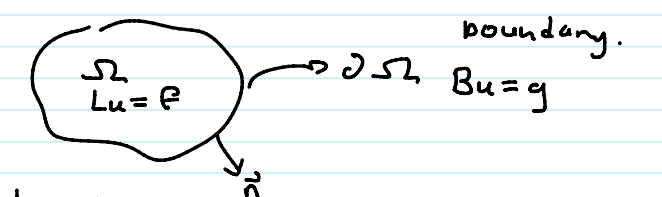
\includegraphics[width = 0.4\linewidth]{Images/elliptic_PDE_setup.png}

\[ \text{Solution domain:} \qquad \Omega\]

\[ \text{Boundary:} \qquad \partial \Omega \]

Look for $u(x,y)$ satisfying

$L u(x,y) = f(x,y)$ on $\Omega$

$L$ -- elliptic differential operator

$f$ -- source/forcing function

$Bu(x,y) = g(x,y)$ on $\partial \Omega$

$B$ -- another operator that encodes BCs

$g$ -- another source function

\vspace{10px}
3 Types of BC's

\begin{enumerate}
    \item Dirichlet - value of u on $\partial R$ is given

    \item Neumann - normal derivative of v on $\partial \Omega $ is given.

    \item Mixed/Robin - some linear combo of $\alpha(x,y)u+\beta (x,y) \frac{\partial u}{\partial x}$ is given.
\end{enumerate}

\subsection{Model Problem}

\begin{itemize}
    \item Poisson equation on unit square with homogeneous Dirichlet Conditions

    \[\nabla ^2 u(x,y) = u_{xx} + u_{yy} = f(x,y) \]

    Subject to 

    \[ u(0,y) = u(1,y) = u(x,0) = u(x,1) = 0\]

    2-1 Discretize Model Problem

    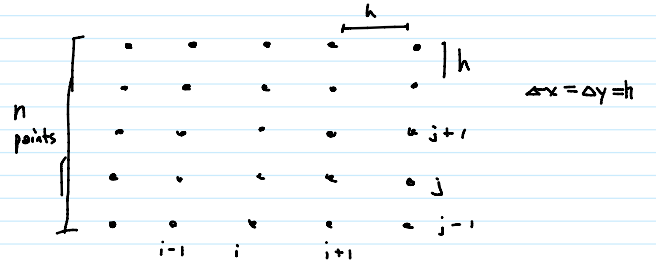
\includegraphics[width = 0.5\linewidth]{Images/model_problem_grid.png}

    \item \textbf{2nd step: }- FDA

    \[ l^h u^h : f^h\]

    \[ B^hu^h: ?\]

    \[ u_{xx} = \frac{u_{i+1,j}-2u_{i,j}+u_{i,j-1}}{h^2} + O(h^2)\]

    \[ u_{yy} = \frac{u_{i+1,j}-2u_{i,j}+u_{i,j-1}}{h^2} + O(h^2)\]

    Substitute into poisson equation

    \[ \frac{u_{i+1,j}+u_{i-1,j}+u_{i,j+1}+u_{i,j-1}-4u{i,j}}{h^2} = f_{i,j} \qquad 2\le i,j\le n-1\]

    where n is the number of points one side

    Discrete BCs
    \[u_{1,j} = u_{n,j} = u_{i,1} = u_{i,n} = 0\]

    using the `plus' stencil

    note that the corner points (0,0), (n,0), (0,n), (n,n) are completely separate due to our stencil choice. But it may be more convenient to just incorporate the points.


    \item \textbf{3rd Step:} How do we solve these equations?

    Write as a linear system

    \[ \mathbf{A} \mathbf{u} = \mathbf{b}\]

    where A has the same sparsity structure as from RD diffusion. Also, its direct solution is expensive, even when accounting for sparsity structure.

    \item Can't us ADI, since (apparently) we can't factor operator into (1-m)(1+m)

    \item A: Use method of relaxation

    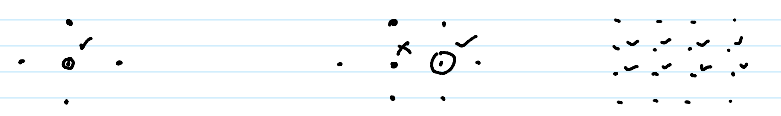
\includegraphics[width = 0.7 \linewidth]{Images/relaxation_stencils.png}
    \begin{enumerate}
        \item plus shape: Instanteously satisfy equation for centerpoint

        \item 2nd one: Move right and satisfy the equation for the next point. Will unsatisfy the previous point in the process! 

        \item large rectangle: Keep going with kick, we get a good solution despite the unsatisfactions (Gauss used this)
    \end{enumerate}
    
\end{itemize}

In his words

\begin{itemize}
    \item Visit each unknown in grid in some order, (row by row, column by column).

    Fix/Freeze other unknowns, adjust our unknown so that its equation is `instantaneously' satisfied.

    \item One complete pass through grid = a relaxation sweep
\end{itemize}

Under certain conditions, this solution will converge.

2 Main ways to update

\begin{enumerate}
    \item Jacobian - use unknowns from previous iteration to satisfy local equations.
    \item Gauss-Seidel - use unknowns most recently computed iteration
\end{enumerate}

We will go over Gauss-Seidel.

\begin{itemize}
    \item Faster
    \item better storage efficiency
    \item basis for successive over relaxation
\end{itemize}

Will also go over way that generalizes immediately to nonlinear equations

Let:

\[ u_{i,j}^{(n)} = \text{discrete solution approx to } u_{i,j} \text{at nth iteration (sweep)} \]

here we assume i sweeps most rapidly

\begin{verbatim}
    for j= 1:n
        for i = 1:n % not those exact indices since only sweeping interior points
\end{verbatim}

\textbf{Residual}

\[ r_{i,j}^{(n)} = h^{-2}(u_{i-1,j}^{(n+1)} + u_{i+1,j}^{(n)} + u_{i,j-1}^{(n+1)}+u_{i,j+1}^{(n)}-4u_{i,j}^{(n)})-f_{i,j}\]

Updates i (right) direction first and then j (up) direction second. This explains the different n-indices in the residual equation.

\textbf{November 17th 11am}

Model Problem (ignoring B.C.'s)

\[ u_{xx} + u_{yy} = f(x,y) \qquad u = u(x,y)\]

Residual for GS relaxation sweep

\[ r_{i,j}^(n) = h^{-2}(u_{i-1,j}^{(n+1)} + u_{i+1,j}^{(n)} + u_{i,j-1}^{(n+1)}+u_{i,j+1}^{(n)}-4u_{1,j}^{(n)})-f_{i,j}\]


\begin{itemize}
    \item Write relaxation in terms of update $\delta u_{i,j}^{(n)}$ and in a way that immediately generatlizes to nonlinear case.

    \[ u_{i,j}^{(n)} \rightarrow u_{i,j}^{(n+1)} = u_{i,j}^{(n)} - r u_{i,j}^{(n)}\]

    \item First define 

    \[ F_{i,j}^h = \frac{u_{i+1,j} + u_{i-1,j}+u_{i,j+1}+u_{i,j-1}-4u_{i,j}}{h^2}-f_{i,j}\]

    \item Newton's Method 

    \[ u_{i,j}^{(n+1)} = u_{i,j}^{(n)} - r_{i,j}^{(n)} \left[ \left. \frac{\partial F_{i,j}^h}{\partial u_{i,j}} \right|_{u_{i,j} = u_{i,j}^{(n)}} \right]^{-1}\]

    \[ u_{i,j}^{(n)} - \frac{r_{i,j}^{(n)}}{-4h^{-2}}\]

    \[ = u_{i,j}^{(n)} + \frac{1}{4} h^2 r_{i,j}^{(n)}\]

    \item Equation above is equivalent to solving other equation directly for $u_{i,j}$ (verify)
\end{itemize}

\subsection{Convergence of Relaxation Methods}
\begin{itemize}
    \item Collect all unknowns $u_{i,j}$ into single vector $\mathbf{u}$ of length $\approx N = n^2$ where $n$ is the number of grid points per grid edge

    \item Write FD equations in matrix form

    \[ \mathbf{A} \mathbf{u} = \mathbf{b}\]

    \item Matrix $\mathbf{A}$ is diagonally dominant if 

    \[|a_{i,j}| \ge \sum_{j=1,j=i}^{N} |a_{i,j}|, \qquad i = 1,2,\ldots , N\]

    \item Rough rule of thumb: GS converges if $\mathbf{A}$ is diagonally dominant (is for current case)

    \item How do we monitor convergence?

    \item Two Natural Approaches

    \begin{enumerate}
        \item Compute Residual Norm: $||mathbf{r}^{(n)}||$

        \item Compute Solution update norm: $||mathbf{u}^{(n+1)}-mathbf{u}^{(n)}||$
    \end{enumerate}

    \item Check so called `running residual' $\Rightarrow$ residuals that appear as we sweep through the mesh

    \item Consider iterative procedure:

    \[ \mathbf{u}^{(0)} \rightarrow \mathbf{u}^{(1)} 
    \rightarrow \ldots
    \rightarrow \mathbf{u}^{(n)} \rightarrow \mathbf{u}^{(n+1)} \rightarrow \ldots \rightarrow \mathbf{0}\]

    \item Errors 
    \[ \mathbf{e}^{(0)} \rightarrow \mathbf{e}^{(1)} 
    \rightarrow \ldots
    \rightarrow \mathbf{e}^{(n)} \rightarrow \mathbf{e}^{(n+1)} \rightarrow \ldots \rightarrow \mathbf{0}\]

    \item For linear relaxation, view transformation or error $\mathbf{e}^{(n)}$ in terms of matrix $\mathbf{G}$ called the error amplification matrix

    \[ \mathbf{e}^{(n+1)} = \mathbf{G}\mathbf{e}^{(n)} = \mathbf{G}^2\mathbf{e}^{(n-1)} = \ldots \mathbf{G}^n \mathbf{e}^{(0)}\]

    \item Asymptotically, convergence is determined by spectral radius $\rho(\mathbf{G})$ of $\mathbf{G}$ where

    \[ \rho(\mathbf{G}) = \text{MAX} | \lambda_i (\mathbf{G})| \]

    where $\lambda$ are the eigenvalues of $\mathbf{G}$

    \item Asymptotic convergence rate R

    \[ R \equiv \log_{10}(\rho^{-1})\]

    \item Interpolation: $1/R =$ the number of sweeps needed asymptotically to decrease $||\mathbf{e}^{(n)}$ by order of magnitude 

    \item For Gauss-Siedel on model Probelm

    \[ \rho(\mathbf{G}_{\text{GS}} = 1-O(h^2)\]

    \[ \Rightarrow 1/R = O(n^2) \Rightarrow \text{\# of sweeps for } ||\mathbf{e}^{(n)} \text{ to decrease by 10}\]

    $\Rightarrow$ total cost $\approx O(N^2) = O(n^4)$

    \item Verify slow convergence; G.S. not useful in practice
    
\end{itemize}

\subsection{Test Solution}

\begin{itemize}
    \item Strategy: specify $u(x,y)$ which satisfies boundary conditions; then compute corresponding RHS function $f(x,y)$

    \[ u(x,y) = \sin(\omega_x x) \sin(\omega_y y)\]

    for $\omega_x$ and $\omega_y$ that are integer multiples of $\pi$

    \item Then 

    \[ f(x,y) = - (\omega_x^2+\omega_y^2) u(x,y)\]

    \item Supply f(x,y) to solution algorithm, should get $u(x,y)$ back (up to truncation error)

    
\end{itemize}

\subsection{Successive Over Relaxation (SOR)}

\begin{itemize}
    \item Historically, researchers found that GS could be sped up by systematically `overcorrecting' updated solutions valves

    $\Rightarrow$ SOR

    \item For model Probelm we have 

    \[ u_{i,j}^{(n+1)} = \omega \hat{u}_{i,j}^{(n+1)} + (1-\omega) u_{i,j}^{(n)}\]

    where u hat is a solution from regular G.S.

    \[ 1 < \omega < 2\]

    for stability 

    \item Under ideal conditions, SOR reduces number of sweeps to $O(n)$. Total cost $O(n^3) = O(N^{3/2}$

    \item When $\rho_{GS}$ can be computed exactly, can compute $\omega_{OPT}$ for model problem 

    \[ \omega_{OPT} = \frac{2}{1+\sin(\pi h)}\]
    
\end{itemize}


\newpage
\def \secname {Stochastic (random) methods}

\section[\secname]{\hyperlink{toc}{\secname}}



\subsection{Overview}

Motivation

\begin{itemize}
    \item Many problems in physics have a non-deterministic or random or stochastic character

    \item Canonical example: Brownian motion; random walk - dynamics of particle subject to some random force

    \item Many other examples: includes almost all statistical mechanical systems

    \item Simulation is often impeded by the need to compute (accurate) expectation values of physical quantities

    \item Consider random walk

    \[ r^2(t^n) \rightarrow \langle r(t^n) \rangle\]

    where $\langle \ldots \rangle$ is average over \textbf{many} trials

    \item sometimes qualitative info can be extracted from small number of simulations
\end{itemize}

Coverage

\begin{itemize}
    \item Uniform random number generators (RNGs)
    \item Non-uniform random number generators
    \item Applications
    \begin{itemize}
        \item Diffusion limited Aggregation
        \item Ising Model
    \end{itemize}
\end{itemize}

\subsection{Pseudo-Random Number Generation (uniform)}

\begin{itemize}
    \item Almost all RNG in computer languages are algorithmic (deterministic); hence terminology `pseudo' RNG (PRNG)

    \item A PRNG can be characterized by a probability distribution function (PDF), p(x) such that 

    \[ p(x) dx \Rightarrow \text{probability that randomly generated number lies in internal x to x+dx}\]

    \item p(x) must be normalized on domain of interest $[x_{min}, x_{max}]$

    \[ \int_{x_{min}}^{x_{max}} p(x) dx = 1\]

    \item Caveat: floating point world is not the continuum, but we are going to ignore that point

    \item p(x) for uniform PRNG

    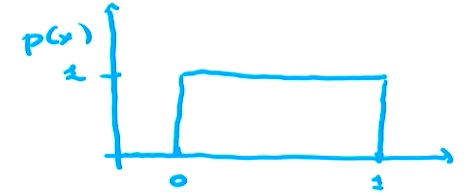
\includegraphics[width = 0.4 \linewidth]{Images/pdf_uniform.png}

    \item Many PRNG algorithms have been developed 

    \item MATLAB provides 9; see held for rng

    \item One common choice, \textbf{Linear Congruential Generator}

    \item Generates sequences of integers whose bit pattern can be interpreted as reals in the range [0,1]

    \[I_{n+1} = (aI_n + c) \text{mod}m\]

    where a and c are other integers and m is an integer called modulus

    \item Good choices for a,c will give maximal period m
\end{itemize}

Seeding a PRNG

\begin{itemize}
    \item MATLAB by design, will return same random number at start-up

    \item Change this behaviour by seeding the RNG. Forces the RNG to start somewhere else in it's sequence

    \item MATLAB

    \begin{verbatim}
        rng(seed)

        % where seed is a non-negative integer
        % same sequence always generated for same seed
    \end{verbatim}
\end{itemize}

\subsection{Pseudo-Random Number Generation (non-uniform)}

\begin{itemize}
    \item Consider some variable (deviate) which is randomly but not necessarily uniformly distributed in some interval $x_{\text{min}} \le x \le x_{\text{max}}$

    Examlpe: Gaussian Distibution ($-\infty < x < \infty$)


    \[ \text{PDF: } p(x) = \frac{1}{\sqrt{\pi \sigma}}e^{-x^2/\sigma^2}\]

    \item Many other examples: poisson, Maxwellian, ...

    \item Given $p(x)$, $x_{\text{min}}$, $x_{\text{max}}$ and a [0,...1] uniform PRNG such as MATLAB's rand, how can we generate deviates distributed according to $p(x)$?

    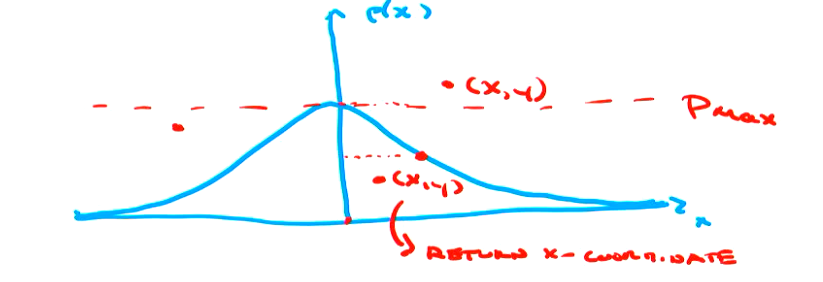
\includegraphics[width = 0.6 \linewidth]{Images/non_uniform_PRNG.png}

    \item Generate random points (x,y) [both coordinates randomly generated] in the region

    \[ x_{\text{min}} \le x \le x_{\text{max}} \]

    \[ y \le p_{\text{max}}\]

    \[ p_{\text{max}} = max(p(x))\]

    $\Rightarrow$ Rejects points that lie above $p(x)$, accepts points below p(x), returning $x$ as the deviate 

    \item Pseudo code for non-uniform PRNG

    \begin{verbatim}
    accept = false
    until accept do
        x = random(xmin, xmax)
        y = random(0,ymax)
        if y<p(x) then rand = x 
        accept = true
        end if
    end do
    \end{verbatim}

    Testing Implementation

    \item Generate large number, n, of deviates on [xmin, xmax]

    \item Compute approximation of PDF p(x) by ``binning" deviates; i.e. count number of deviates in each interval/bin

    \[ x_i \text{ to } x_i+\Delta x\]

    \[ x_1 = x_{\text{min}}\]

    \[ x_N = x_{\text{max}}\]

    \[ \Delta x = \frac{x_{\text{max}}-x_{\text{min}}}{N_1}\]

    \[ N-1 = \text{ \# of bins}\]

    \item Normalization (verify) let $c_i$ be the count for the i-th bin, then

    \[ \bar{c}_i = \frac{c_i}{n\Delta x}\]

    And 

    \[ lim_{n\rightarrow \infty , N \rightarrow \infty} \bar{c}_i = p(x_i)\]
    
\end{itemize}

\subsection{Diffusion Limited Aggregation (DLA)}

Model for growth of clusters $\Rightarrow$ collections of identical particles

Examples:

\begin{enumerate}
    \item Snow Flakes
    \item Soot particles
    \item Frost (Hoar Frost)
    \item Lightning; sparks
    \item Urban growth
\end{enumerate}

\begin{itemize}
    \item These clusters (aggregates) are characterized by dendritic (branching) structure

    \item Typically have non-integer dimensionality (fractal)

    \[ m(r) = \text{mass contained within radius r}\]

    \[ m(r) = r^d \rightarrow \text{fractal dimension}\]

    \[ \text{Typically} \quad 1 < d < 2\]
\end{itemize}

DLA Algorithm 

\begin{itemize}
    \item Use 2-D uniform lattice in (x,y)

    Particles: unit mass; two types

    \begin{itemize}
        \item Fixed/ Frozen: structure at some specific lattice site
        \item Mobile: free to random walk on lattice
    \end{itemize}

    Discrete time steps $t^n$

    Simplest Implementation

    \begin{itemize}
        \item One free particle at any time
        \item Particle random walks until becomes adjacent to a lattice site with fixed particle
        \item Free particle gets frozen at current position
        \item New random walker is launched
        \item Cluster: all fixed particles
    \end{itemize}

    Growth is \textbf{SLOW}

    \[ D_{\text{RMS}} = \langle D^2 \rangle^{\frac{1}{2}} \tilde n^\frac{1}{2}\]

    where n is the number of steps

    Extension: central bias

    \[ 0 \le b \le 1\]

    \[ b: \text{ Probability that walker takes extra step directly toward the center}\]

    \item Using the bias we can speed up the computation but it makes the fractal more clumpy and concentrated at the center. 
\end{itemize}

\textbf{missed friday class}



\textbf{November 27th 2023 11:06am (caught up)}

Recall: Monte Carlo Method (ISING system)

\begin{verbatim}
    if E_flip <= 0
        flip spin
    else 
        generate r = random(0,1)
        if re = exp(-E-flip((kBT)))
            flip spin
        else 
            leave spin as is
        end
    end
\end{verbatim}

\[ \Rightarrow \frac{P_1}{P_2} = \exp[-(E_1-E_2)/(k_BT)]\]

$\Rightarrow$ what is needed for thermal equilibrium?

\subsection{Physical Behaviour of Model}

\begin{itemize}
    \item System characterized by \textbf{competition}
    \begin{itemize}
        \item Ferromagnetic interaction tends to \textbf{order} system (spin alignment favoured as $T\rightarrow0$)
        \item Temperature tends to disorder system (spin completely randomized at high T)
    \end{itemize}
    \item At some critical temperature ($T_c$) and in the thermodynamic limit ($N\rightarrow\infty$) there will be a phase transition
\end{itemize}

Physical Quantities to measure (expectation values)

\begin{itemize}
    \item When simulating, need to give system time to equilibrate; then run for long enough to generate ``good statistics"
    \item Make passes through lattice; each pass generates new microstate $\alpha$; compute expectation values by averaging over these states
    \item Typically normalize quantities by dividing by number of spins
    \begin{itemize}
        \item Average energy $\langle E \rangle $
        \item Avergae magnetization $\langle M \rangle $
    \end{itemize}

    \[ E = - J \sum_{\langle ij\rangle} s_i s_j (-\mu H \sum_i s_i\]

    \item At T=0 (Take J=1); what is $\langle E \rangle$?

    \[ \langle E \rangle = -2J = -2; \]

    each spin contributes -4J;
    Divide by 2 to account for double-counting

    \item As $T\rightarrow \infty$, what is $\langle E \rangle$?

    \[ \langle E \rangle \rightarrow 0;\]
    But have to go to quite high T to see this since correlations among spins persist for even high T
\end{itemize}

Derived Quantities
\begin{itemize}
    \item Consider Variance of Energy

    \[ (\Delta E ) ^2 \equiv \langle E^2 \rangle - \langle E \rangle^2\]

    \item Fluctuation-Dissipation theorem (connects fluctuations to response of system to external perturbation). Relates to specific heat.

    \[ C = \frac{(\Delta E)^2}{k_B T^2}\]

    Will work in units where $k_B=1$

    \item Similarly, variance in M is related to susceptibility $\chi = \frac{dM}{dH}$ ($H\equiv$ Magnetic field)

    \[ \chi = \frac{(\Delta M)^2}{k_B T}\]

    Behaviour near $T=T_c$

    \item Scaling of Magnetization

    \[ M \sim (T-T_c)^{\beta}\]

    $\beta \rightarrow$ universal exponent

    \begin{center}
        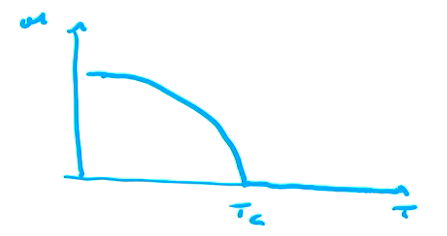
\includegraphics[width = 0.5\linewidth]{Images/ising_phase_transition.png}
    \end{center}

    \item exact solution of 2D ISING model (onsager 1944)

    \[ T_c = \frac{2}{ln(1+\sqrt{2}} = 2.2692 \ldots \]

    \[ \beta = \frac{1}{8}\]

    \item C and $\chi$ are divergent at $T=T_c$

    \item Phasee transition for $M=0$ is called second order or continuous since the order parameter $\langle M \rangle$ does not have a jump at $T=T_c$
    
\end{itemize}

\subsection{Behaviour of Model for $H\neq 0$}

\begin{itemize}
    \item Now have 2 extensive parameters: T, H

    \item Phase Diagram

    \begin{itemize}
        \item For low T, $T<T_c$, per spin magnetization is $<0$ on one side and $>0$ on other
    \end{itemize}

    \begin{center}
        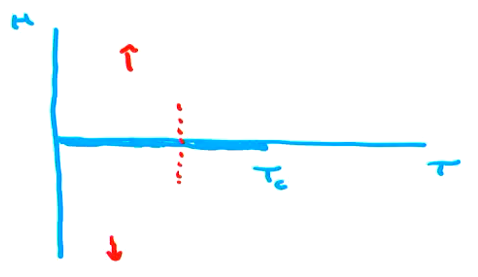
\includegraphics[width = 0.5\linewidth]{Images/H0_ising.png}
    \end{center}

    \item Thus, have a discontinuity in $\langle M \rangle $ as we tune across H=0
    \begin{center}
        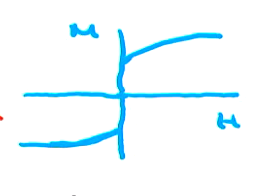
\includegraphics[width = 0.5\linewidth]{Images/MH_ising.png}
    \end{center}

    \item $\Rightarrow$ first order phase transition 
    \item Line in T-H plane 
    \item Above $T_c$ there is no spontaneous magnetization so no possibility of discontinuity in $\langle M \rangle$ as H passes through 0
    
    \item Phase transition line terminates at critical point

    $\Rightarrow$ general feature of first-order phase transition
    
\end{itemize}


\subsection{Phase Transitions}

\begin{center}
    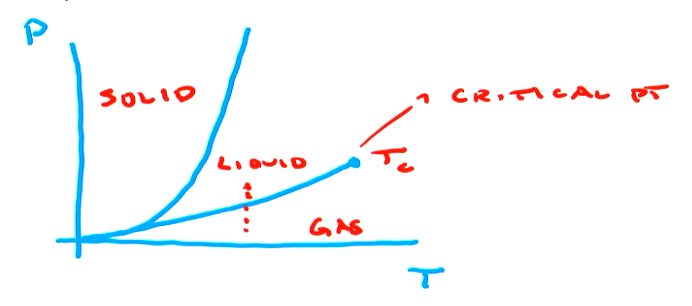
\includegraphics[width = 0.5\linewidth]{Images/phase_transtion_PT.png}
\end{center}

\begin{itemize}
    \item Similar situation: Gas-Liquid System: First order over a range of pressures, with a discontinuity in density
    \item As P increase, size of discontinuity decreases, vanishes at critical point
    \item Key difference between second order, first order phase transitions
    \begin{itemize}
        \item Second order: fluctuations become large near transition.
        \item First order: No growth in fluctuation near transition; happens suddenly
    \end{itemize}

    \item $\langle M \rangle $ vs H for ISING system can exhibit hysteresis, especially at low T
\end{itemize}


\newpage
\def \secname {Fourier Transform}

\section[\secname]{\hyperlink{toc}{\secname}}



(following Numerical Methods, Press et al.)

\subsection{Quick Review}

\begin{itemize}
    \item Transform pairs: $h(t) \Longleftrightarrow H(f)$

    \[ h(at) \Longleftrightarrow \frac{a}{|a|} H(\frac{f}{|H|}\]

    \item Convolution

    \[ g*h \equiv \int_{-\infty}^{\infty} g(\tau) h(t-\tau)d\tau\]

    \[ g*h \Longleftrightarrow G(f)H(f) \quad \text{Convolution Theorem}\]

    \item Total Power 

    \[ \int_{-\infty}^{\infty} |h(t)|^2dt = \int_{-\infty}^{\infty} |H(f)|^2 df\]

    Parseval's Theorem

\end{itemize}

\subsection{FT of Discretely Sampled Data}

\subsubsection{Sampling Theorem and Aliasing}

\begin{itemize}
    \item Assume $h(t)$ sampled uniformly in time

    \[ h_n = h(\Delta n), \quad n=\ldots,-1,0,1,\ldots\]

    \item Sampling Rate: $\frac{1}{\Delta}$

    \item Nyquist Critical Frequency: $f_c = \frac{1}{2\Delta}$

    \begin{center}
        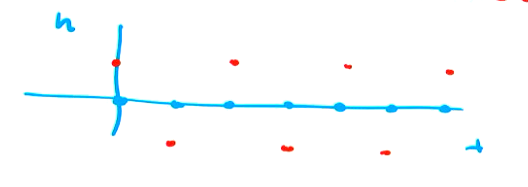
\includegraphics[width = 0.5 \linewidth]{Images/nyquist_aliasing.png}
    \end{center}

    \item Sampling Theorem: If continuous function h(t), samples at interval $\Delta$, its bandwidth limited to frequencies smaller than $f_c$ ($H(f) = 0$ for all $|f| \ge f_c$) then function is completely determined by its samples $h_n$

    \[ h(t) = \Delta \sum_{n=-\infty}^{+\infty} h_n \frac{\sin(2\pi f_c(t-n\Delta)}{\pi(t-n\Delta)}\]

    \item What happens if function is not bandwidth limited?

    \item All power spectral density outside nyquist range $-f_c < f < f_c$ is moved into that range $\Rightarrow$ \textbf{Alisasing}.

    \item Two waves exp($2\pi f,t$) and exp($2\pi f_c t$) yield same samples if and only if f, and $f_c$ by multiple of $\frac{1}{\Delta} \rightarrow$ width in frequency of range ($-f_c,f_c$)
\end{itemize}

\subsubsection{Discrete Fourier Transform}

\begin{itemize}
    \item Now what to estimate Fourier transform if a function from finite number of sample points.
    \item Suppose we have

    \[ h_k \equiv h(t_k), \qquad t_k = k\Delta, \quad k=0,1,\ldots, N-1\]

    Where $Delta$ is the spacing and $N$ is the number of samples.

    \item Will assume that N is even

    \item Seek estimates at discrete values

    \[ f_n = \frac{n}{N\Delta}, \qquad n = \frac{-N}{2}, \ldots , \frac{N}{2}\]

    \item Extreme values $\rightarrow$ lower and upper limits of the Nyquist critical frequency range

    \item Estimates for $n=-N/2,$ $N/2$ are equal $\Rightarrow$ there are a total of N independent $H_n$

    \[ H(f) = \int_{-\infty}^{\infty} h(t) e^{2\pi i f t} dt\]

    \item Approximate using discrete sum

    \begin{align}
        H(f_n) &= \int_{-\infty}^{\infty} h(t) e^{2 \pi i f_n t} \approx \sum_{k=0}^{N-1} h_k e^{2\pi i f_n t_n} \Delta \\
        &= \Delta \sum_{k=0}^{N-1} h_k e^{2\pi i k_n/N} 
    \end{align}

    \item Defines discrete Fourier Transform

    \begin{equation}
        H_n = \sum_{k=0}^{N-1} h_k e^{2\pi i k_n/N} 
    \end{equation}

    \item Have 

    \[ H(f_n) \approx \Delta H_n\]

    \item n value from -N/2 to N/2

    \item equation above is periodic in n with period N

    \[ \Rightarrow H_{-n} = H_{N-n}, \qquad n=1,2,\ldots\]

    \item Useful convention, let n take on values 0,1,2,..., N-1

    \begin{itemize}
        \item Zero frequency: n=0
        \item Positive frequency: n=1,2,...,N/2-1
        \item Negative frequency: n=N/2+1,N/2+2,...,N-1

        For Total of N samples 
        
    \end{itemize}

    \item Discrete inverse Fourier transform

    \[ h_k = \frac{1}{N} \sum_{n=0}^{N-1} H_n e^{-2 \pi i k_n/N}\]

    \item Discrete version of Parseval's Theorem

    \[ \sum_{k=0}^{N-1} |h_n|^2 =  \frac{1}{N} \sum_{n=0}^{N-1} |H_n|^2\]
\end{itemize}

\subsubsection{Fast Fourier Transform}

\begin{itemize}
    \item How much computation does it take to evaluate equation (73) above?

    \item Define complex number

    \[ w = e^{2\pi i/N}\]

    \item (73) can be written as

    \[ H_n = \sum_{k=0}^{N-1} w^{nk} h_k \]

    (exponent gives: nk-th power of w)
    
    \item In vector-matrix form

    \begin{equation}
        \mathbf{H} = \mathbf{A} \mathbf{h}
    \end{equation}

    \[ A_{ij} = w^{ij}\]

    \item (74) take $N^2$ multiplications and somewhat fewer operations to compute all $w^{ij}$

    \item Can actually evaluate FT in $O(N \ln N)$ operations $\Rightarrow$ Fast Fourier Transform $\Rightarrow$ FFT

    \item Key observation (Danielson; Lankzos in 1942, but many others before, including Gauss) 

    \[ F_k = F_k^{\text{e}} + w^k F_k^{\text{o}}\]

    \[ e \equiv \text{even}\]
    \[ o \equiv \text{odd}\]

    Can be applied recursively to $F_k^e$, $F_k^o$ all the way to single samples if N is a power of 2.

\end{itemize}

\end{document}